% \section{Software Requirements Specification}

\section{Einführung}

\subsection{\textbf{Zweck}}
Dieses Dokument dient als Dokumentation des berufsbegleitenden Studienganges, Kommunikations- und Medieninformatik des Matrikel 13, mit der Programmierung einer APP zur Kompression von Bilddaten. Es setzt dabei die Rahmenbedingungen fest.

\subsection{\textbf{Hintergründe und Ziele des Projekts}}
Die \acf{HfTL} ist eine private, staatlich anerkannte Fachhochschule. Träger der \ac{HfTL} ist die \ac{HfTL}-Trägergesellschaft \acs{mbH}, eine Beteiligungsgesellschaft der Deutschen Telekom AG. Die Hochschule befindet sich im Leipziger Stadtteil Connewitz. Es werden sowohl Direkt- als auch duale Studiengänge und berufsbegleitende Studiengänge angeboten.

\subsection{\textbf{Produktumfang}}

Der Betrieb der Smartphone-APP muss auf allen gängigen Android-Smartphones ab Version 4.4.2 möglich sein.

Durch die APP wird den Studenten der HFTL ermöglicht: 

\begin{itemize}
      \item Fotos aufnehmen
      \item Bilder mit einer skalaren Quantisierung komprimieren
      \item Quantisierungsinterval soll einstellbar sein 
      \item Ablage der komprimierten Bilder in passend zum Verfahren benannten Ordnern
\end{itemize}
   



\subsection{\textbf{Musskriterien}}

Zunächst müssen zwingend folgende Punkte des Umfangs erfüllt werden:

\begin{itemize}
   	\item Bildaufnahme
   	\item Quantisierung
   	\item Auswahl Quantisierungsinterval
   	\item Abspeichern mit passendem Dateinamen 
\end{itemize}

\subsection{\textbf{Abgrenzungskriterien}}

Die \acs{APP} soll später auch um zusätzliche Funktionen, wie Vektorquantisierung oder andere Verfahren erweiterbar sein. Versionen für andere Betriebssysteme müssen in einem seperaten Projekt bearbeitet werden und sind nicht Bestandteil dieses Projektes.			

\subsubsection{Kostenrahmen}

Für die Entwicklung der \acs{APP} soll auf kostenfreie Opensource-Programme oder auf vordefinierte Klassen für die Programmierung zurückgegriffen werden.


\subsection{\textbf{Definitionen, Akronyme, Abkürzungen}}
\begin{acronym}[UV-Licht]
\acro{HfTL}{Hochschule für Telekommunikation Leipzig}
\acro{APP}{Kurzform für Applikation}
\acro{mbH}{mit beschränkter Haftung}
\acro{QIS}{Qualitätssteigerung der Hochschulverwaltung im Internet durch Selbstbedienung}
\acro{iCal}{Datenformat zum Austausch von Kalenderinhalten}
\acro{SoSe15}{Sommersemester 2015}
\acro{XML}{ Extensible Markup Language}
\acro{HTTPS}{HyperText Transfer Protocol Secure}
\acro{AES}{Advanced Encryption Standard}
\acro{SQL}{Structured Query Language}
\acro{.apk}{Android application package}
\acro{MTBF}{mean time between failure}
\acro{CI/CD}{Corperate Identity/Corperate Design}
\acro{GUI}{Graphical User Interface}
\acro{QuantiPig}{quantisiertes Picture}


\end{acronym}

%\subsection{\textbf{Referenzen}}
%
%\begin{itemize}		
%	\item QIS-System:  \url{https://qisweb.hispro.de/tel/rds?state=user&type=0} 
%	
%	\item News der HfTL  \url{https://www.hft-leipzig.de/de/studierende/service/news.html}	
%\end{itemize}


\section{Allgemeine Übersicht}

\subsection{\textbf{Beschreibung der Ausgangssituation (Ist-Zustand) }}

Als Ausgangssituation wurden der Studentengruppe drei \acs{APP}'s aus vorherigen Matrikeln vorgelegt, die ebenfalls Bilddaten komprimieren. Diese drei \acs{APP}'s gilt es zu vergleichen und die Stärken herauszuarbeiten. Anhand dieser Ergebnisse gilt es eine neue \acs{APP} zu entwickeln.


\subsubsection{Vergleich der vorhandenen drei \acs{APP}'s}
\begin{landscape}
%\begin{tabular}{| l | p{5cm} | l | l |}
%\hline
%\textbf{Punkte} & \textbf{PhotoQuant} & \textbf{QuantiPic} & \textbf{QuanPic} \\
%\hline
%\textbf{Merkmale} & drei Modi (Lloyd-Algo,Midthread,Originalbild) & drei Modi (Original,Farbwerte,Helligkeit) & zwei Modi (Original,MedianBlur)\\
%\hline
%\textbf{Auflösung} & 2688x1520 px & 1456x832 px & 1456x832 px \\
%
%\hline
%\textbf{Speicherformat} & JPEG & .png & .png \\
%
%\hline
%\textbf{Vorteile} & \begin{itemize}
%\item APP speichert Bilder je nach Verfahren in einem spezifischen Ordner
%\item setzt Zeitstempel bei Bildern
%\end{itemize} dlfkjsdlfjh & lskjfdlasjdf \\
%
%
%\hline
%\textbf{Nachteile} & dsjföskdjf & dlfkjsdlfjh & sldkjfldskjfh\\
%\hline
%
%\textbf{Usability} & dsjföskdjf & dlfkjsdlfjh & lkjdsflajsd\\
%\hline
%
%
%\end{tabular}

\newpage

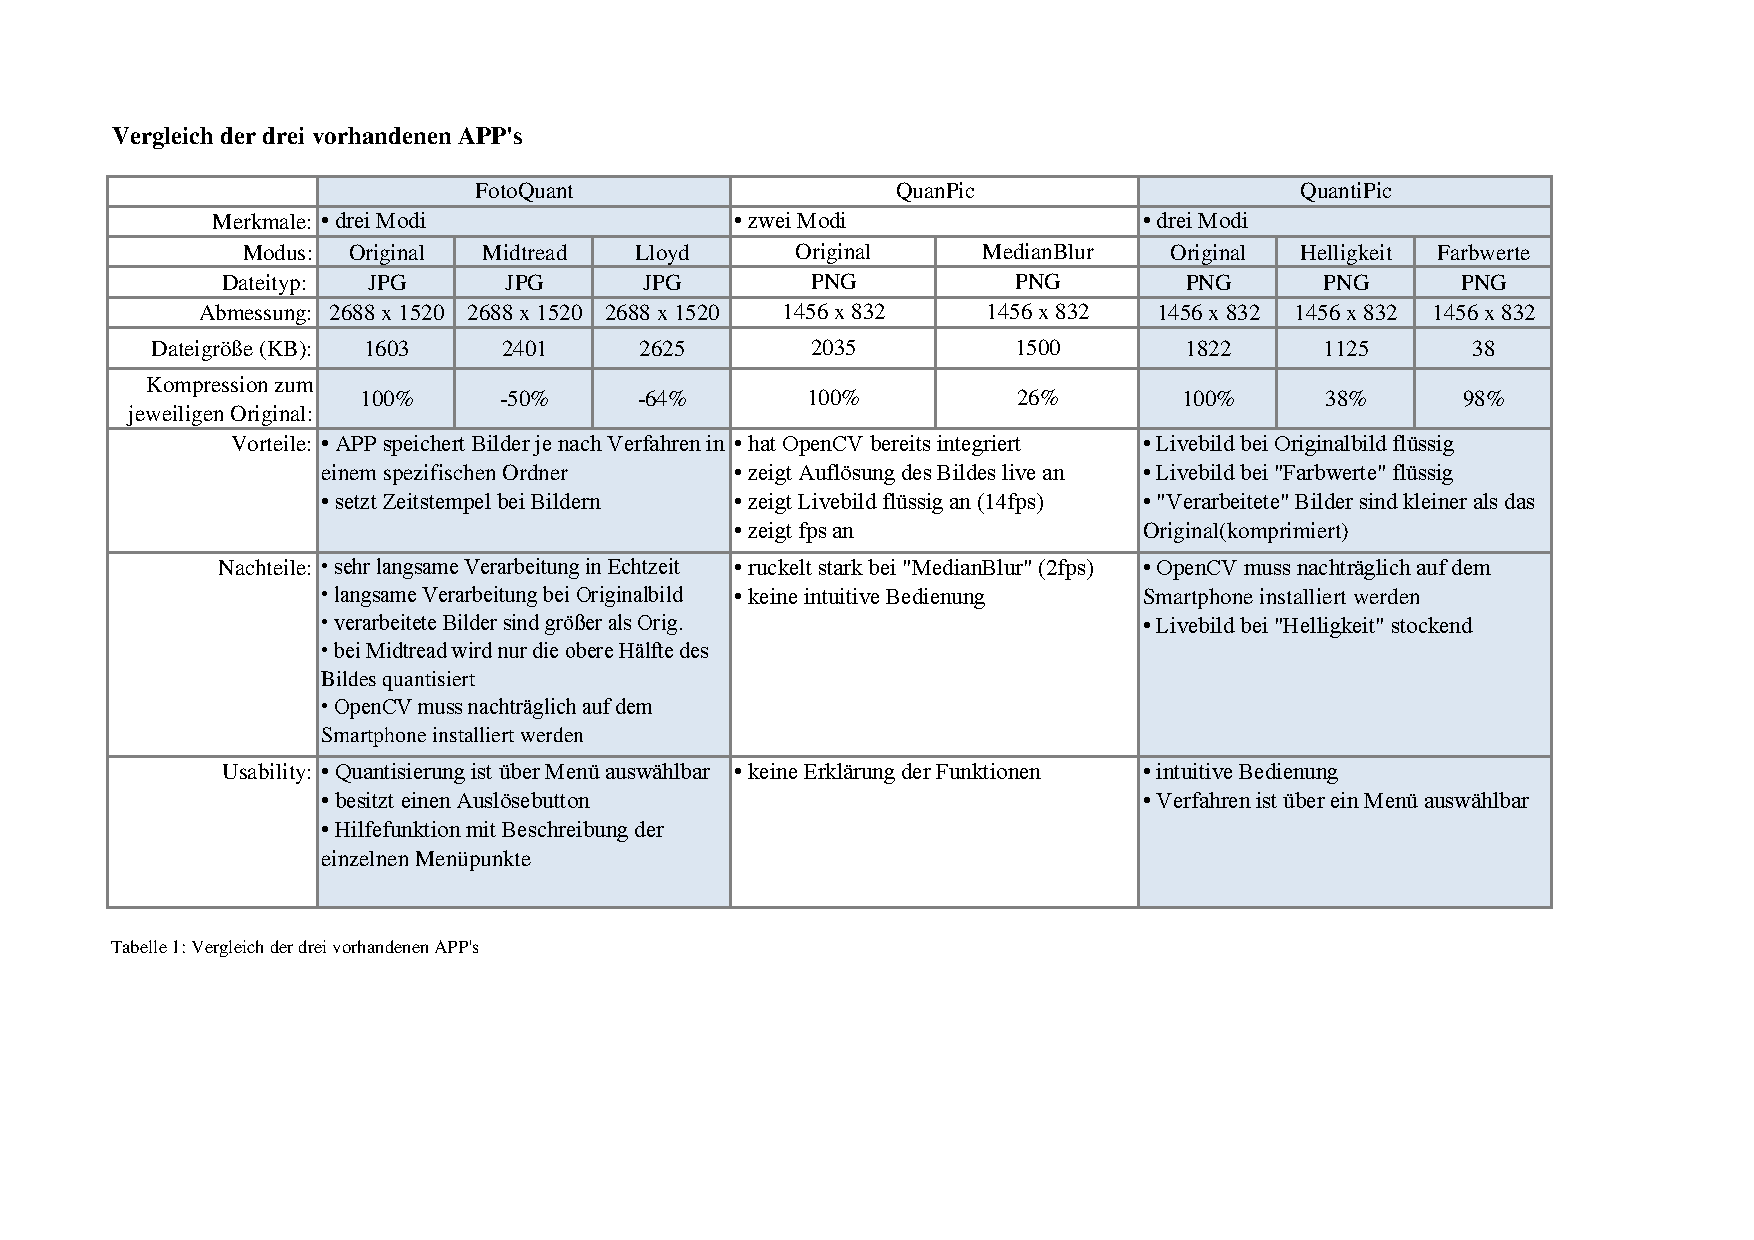
\includepdf[landscape=true,pages=-,noautoscale]{04_Anhang/files/Vergleich_Apps.pdf}

\end{landscape}


\subsection{Beispielbilder}

\begin{landscape}

\begin{figure}[h]
	\centering
		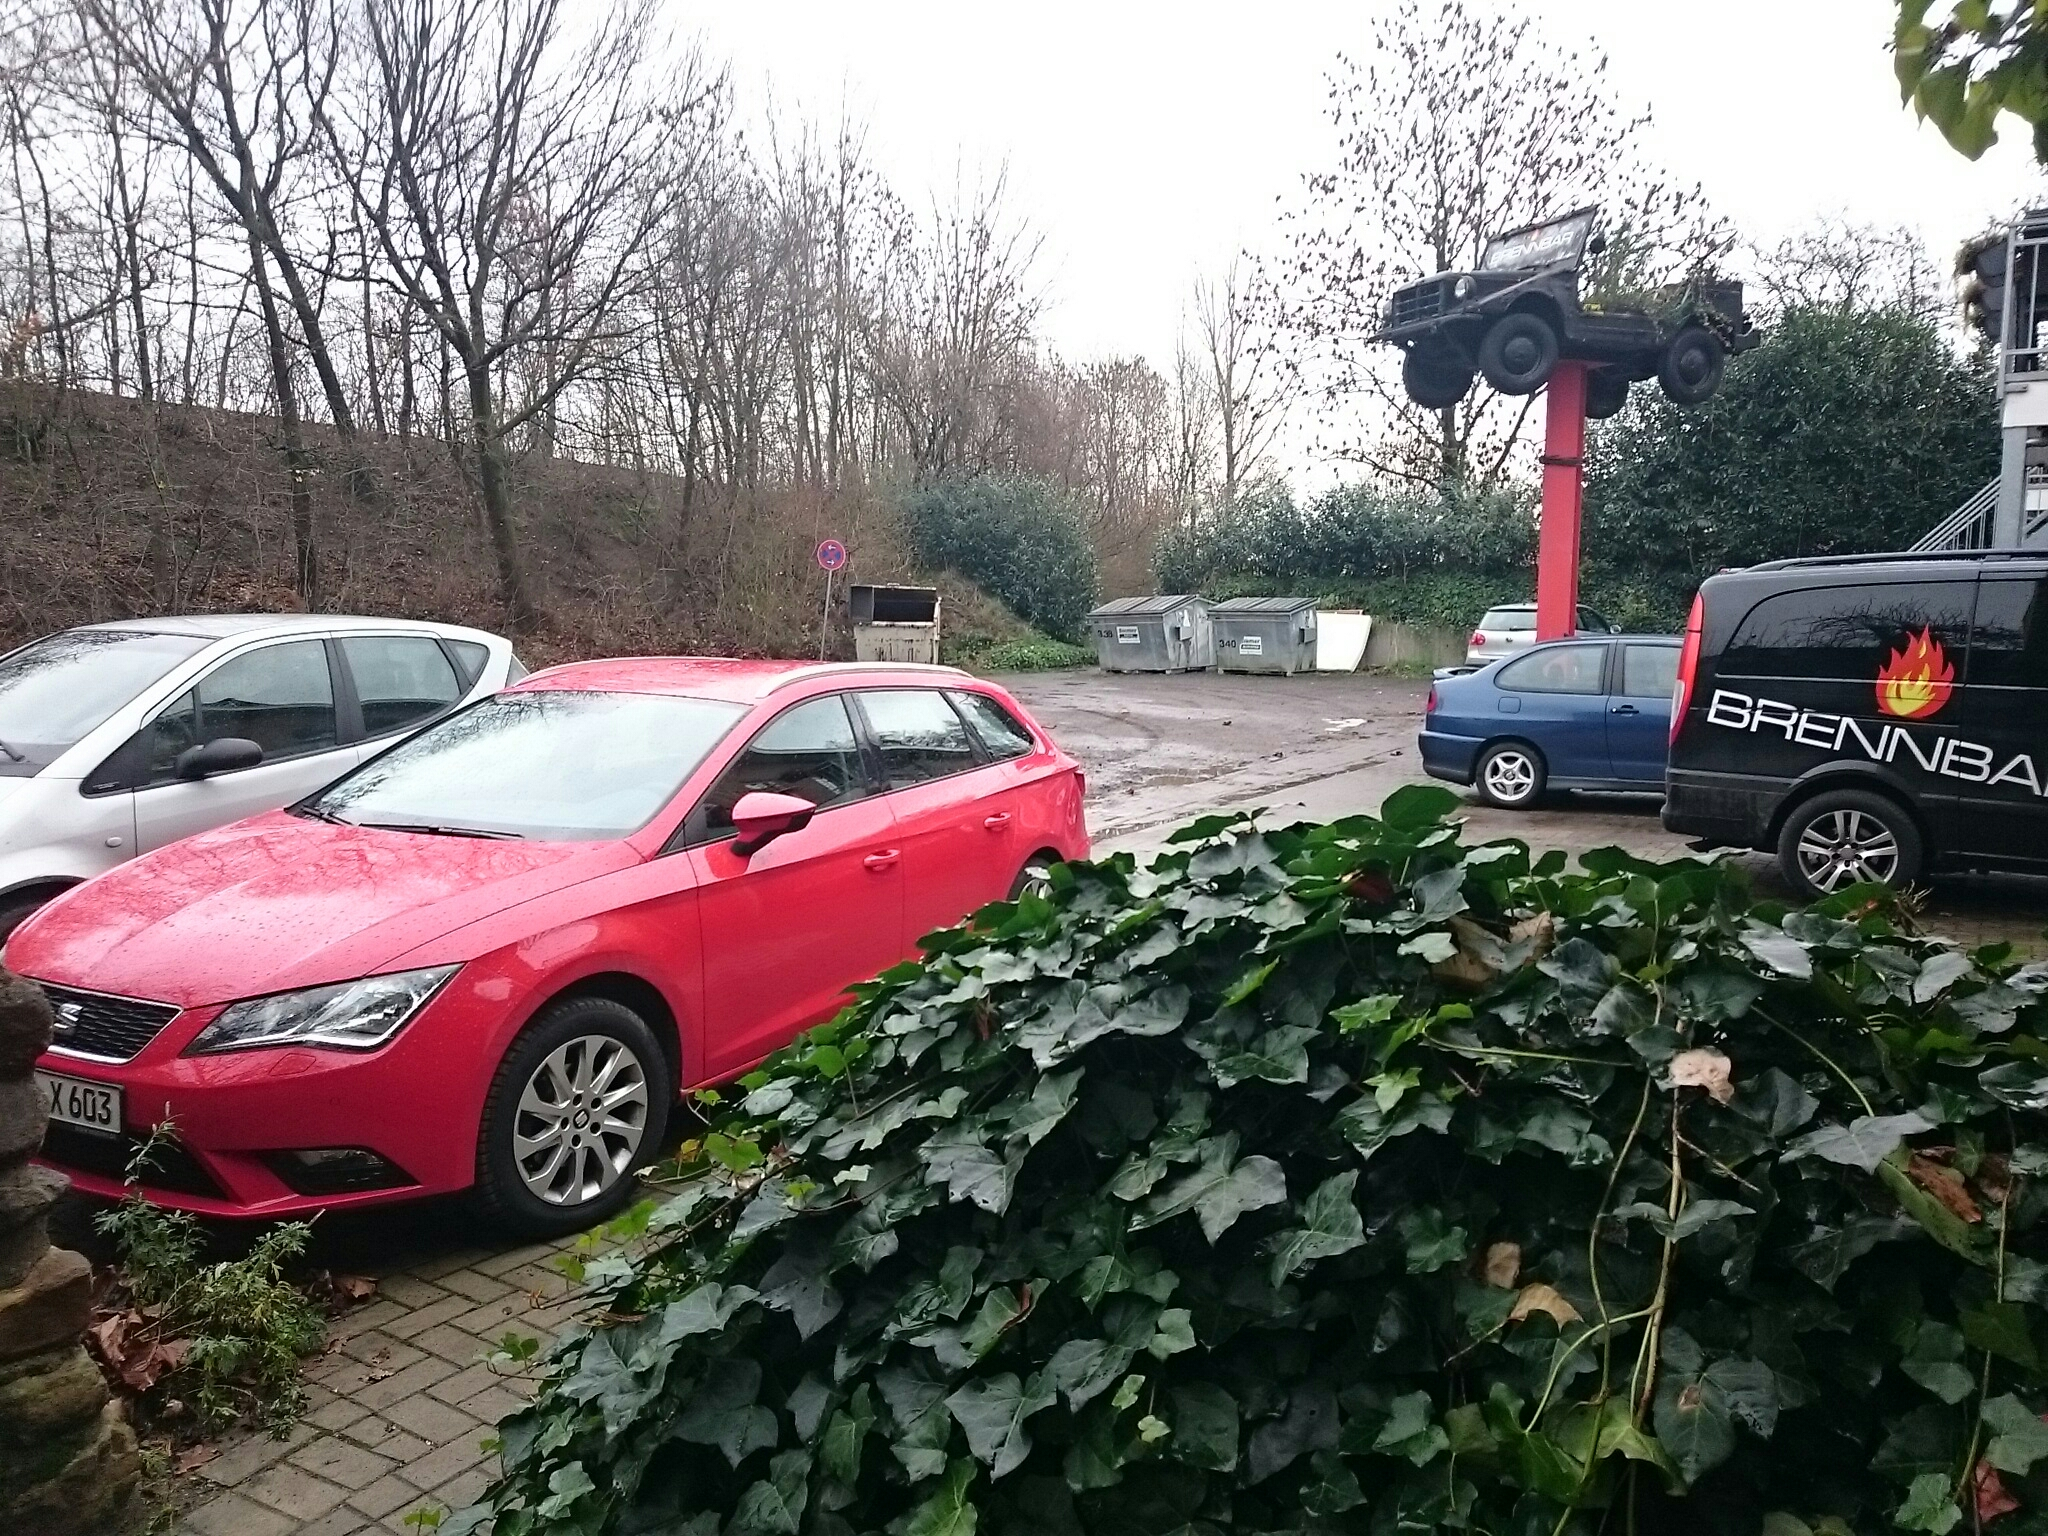
\includegraphics[width=1.4\textwidth]{img/Fotos/FotoQuant_Original.jpg}
	\caption[PhotoQuant Original]{PhotoQuant Originalbild}
	\label{fig:quant_ori}
\end{figure}



\begin{figure}[h]
	\centering
		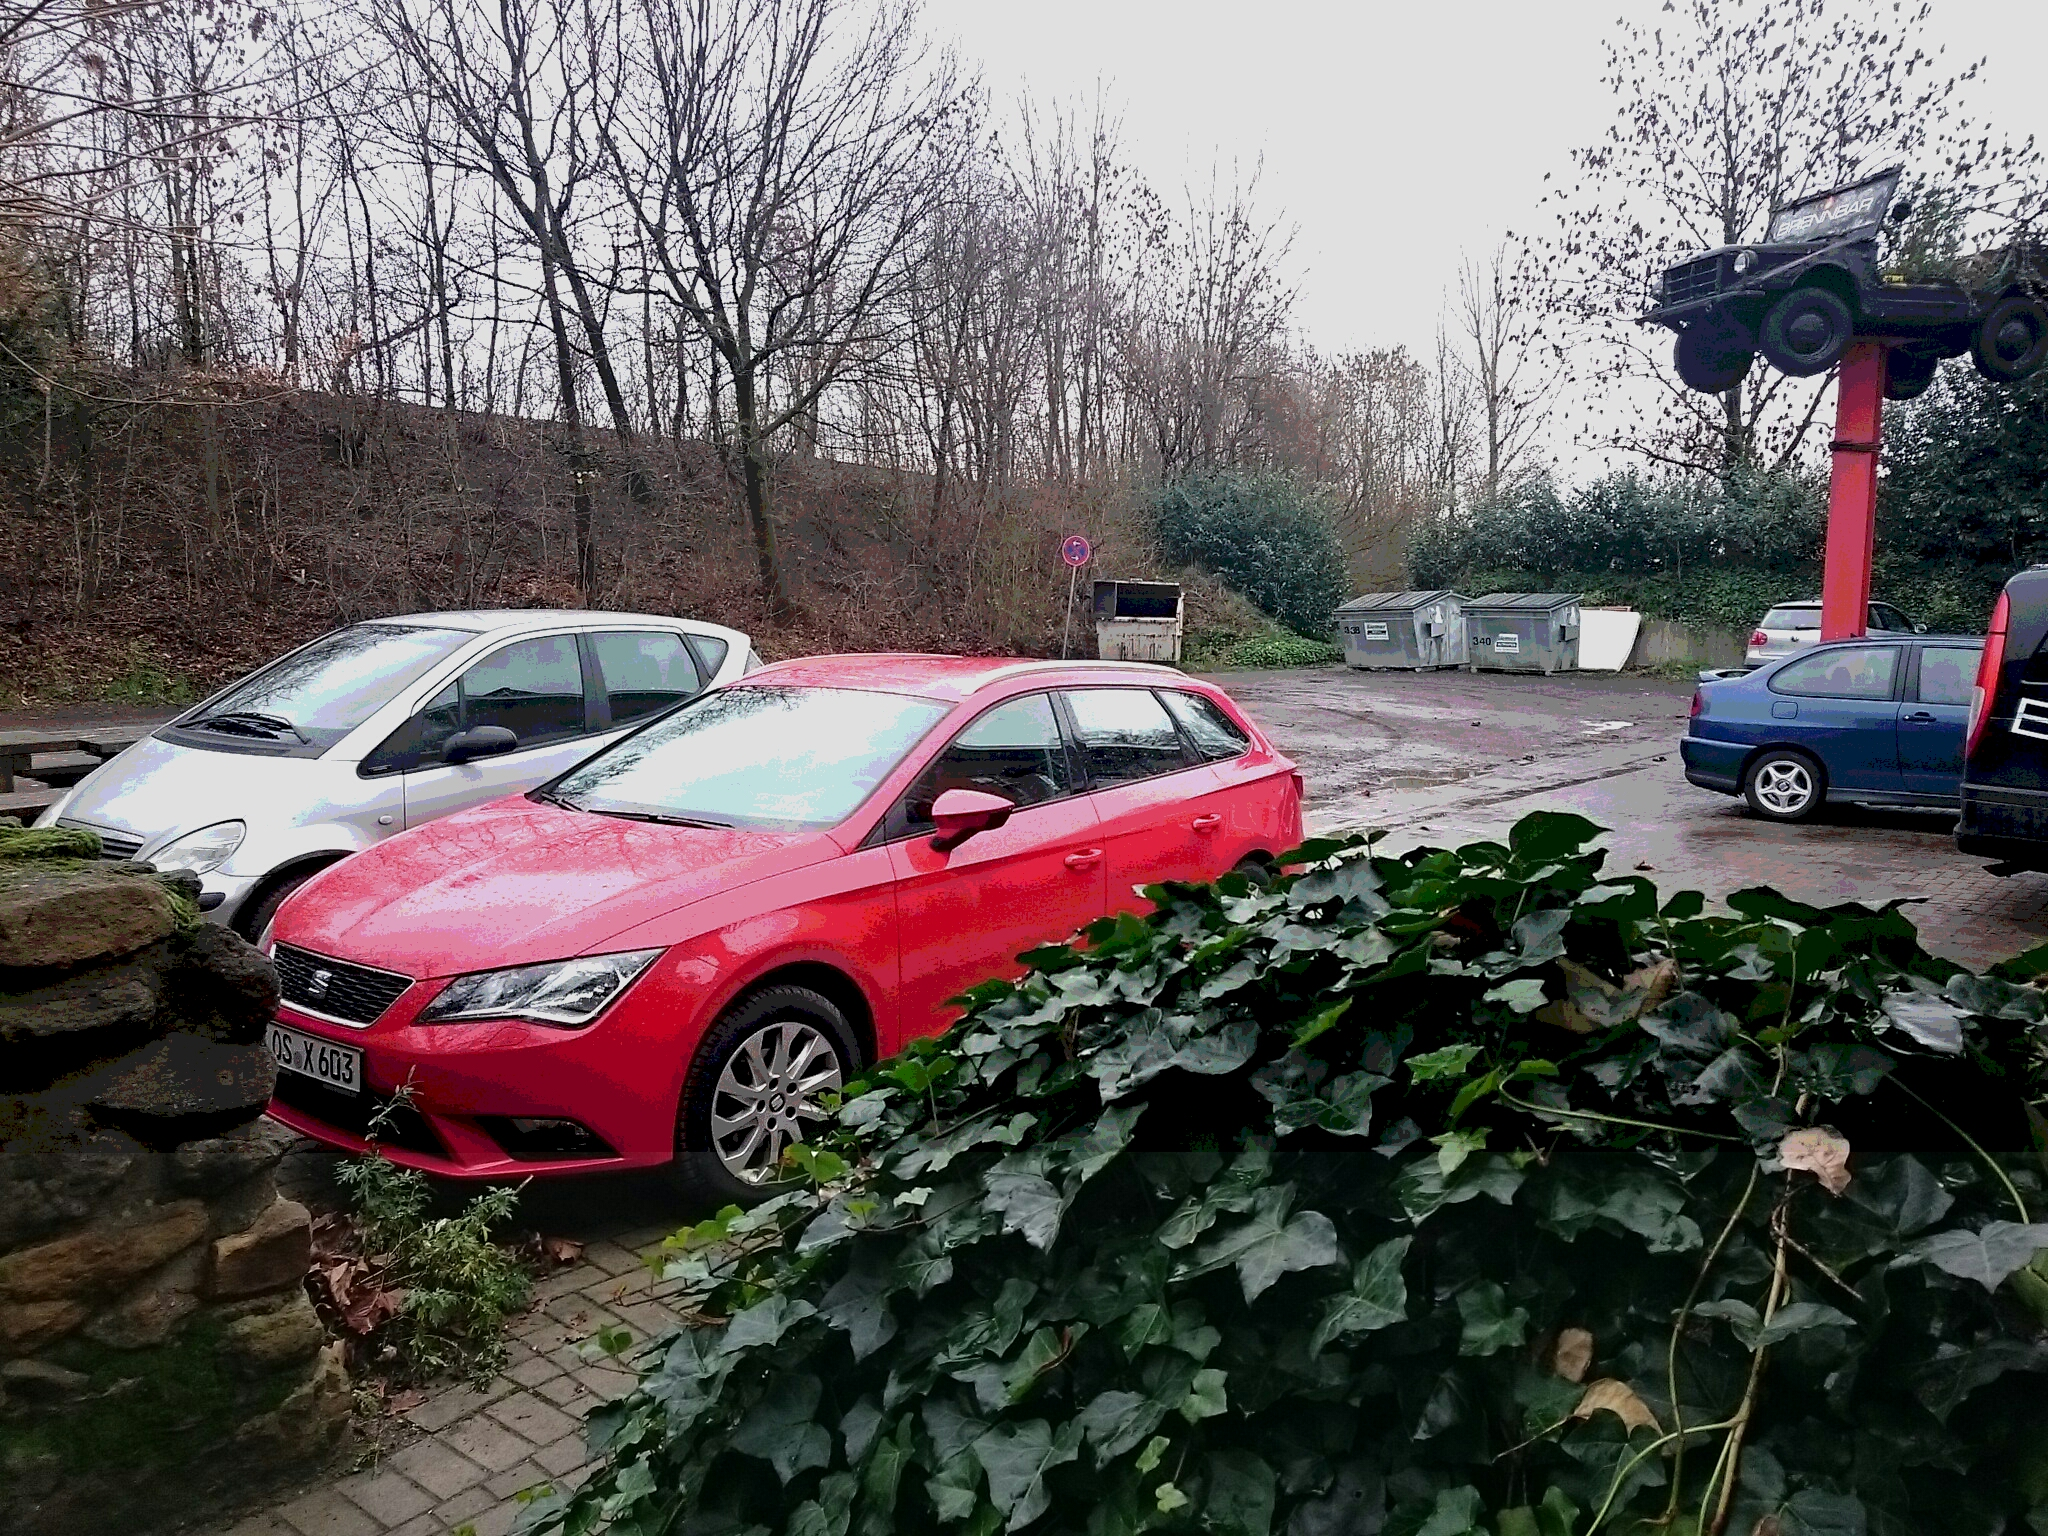
\includegraphics[width=1.4\textwidth]{img/Fotos/FotoQuant_Midtread.jpg}
	\caption[PhotoQuant MidTread]{PhotoQuant MidTread-Modus}
	\label{fig:quant_mid}
\end{figure}

\begin{figure}[h]
	\centering
		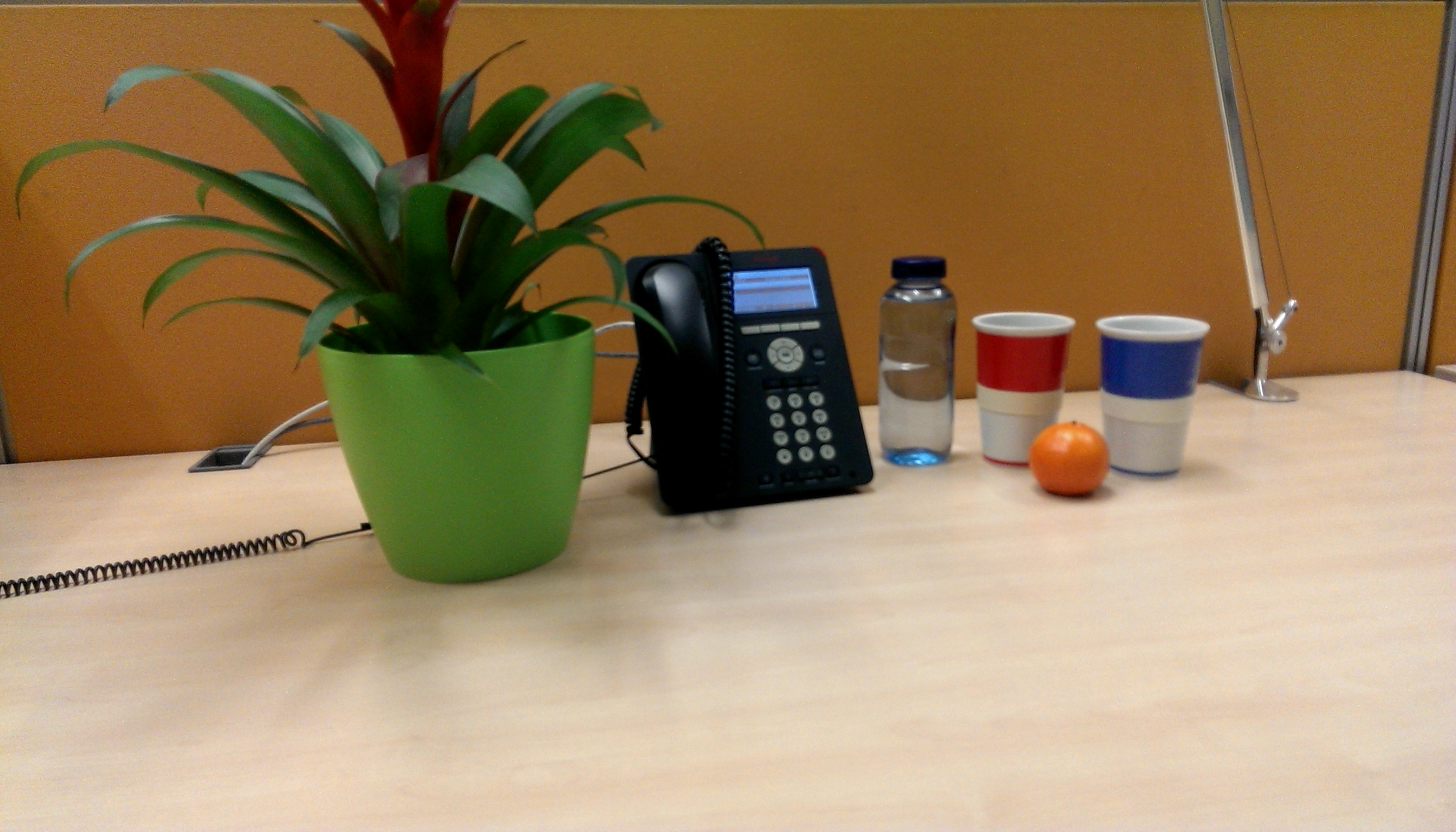
\includegraphics[width=1.4\textwidth]{img/Fotos/QuanPic_Original.png}
	\caption[QuanPic Original]{Quanpic im Originalbild-Modus}
	\label{fig:quan_orig}
\end{figure}

\begin{figure}[h]
	\centering
		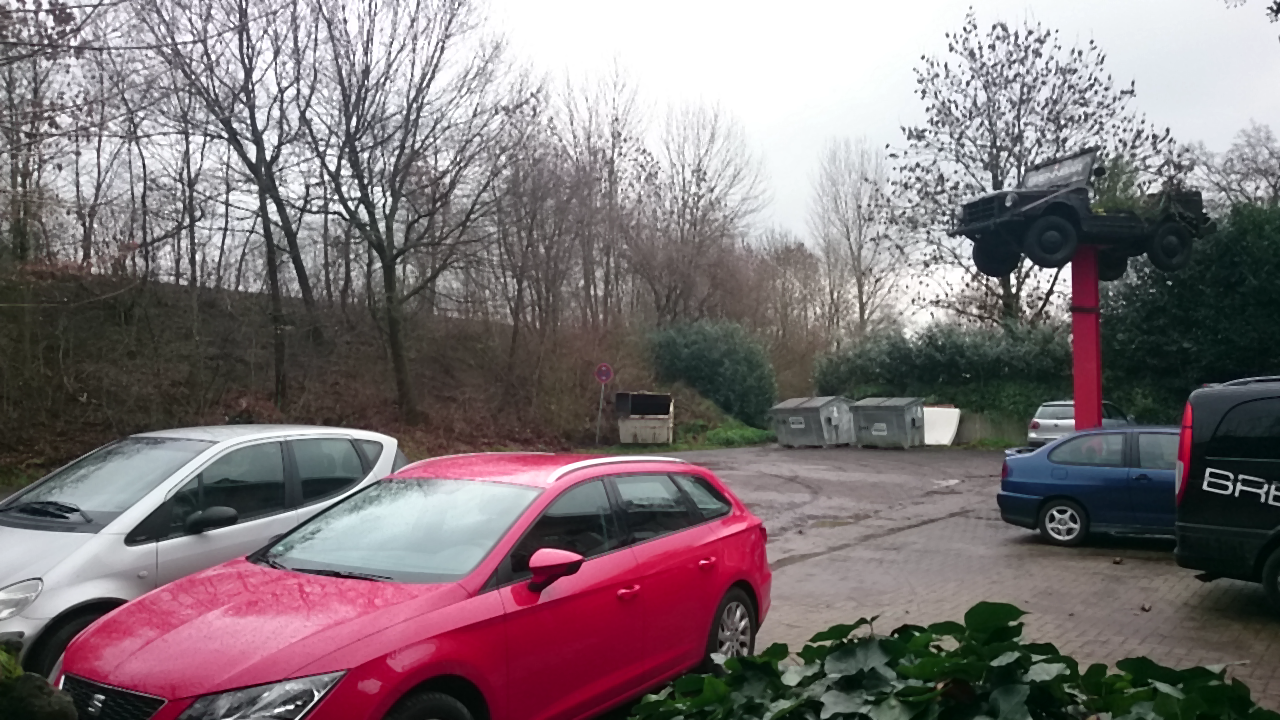
\includegraphics[width=1.4\textwidth]{img/Fotos/QuanPic_Medianblur.png}
	\caption[QuanPic MedianBlur]{Quanpic im MedianBlur-Modus}
	\label{fig:quan_med}
\end{figure}

\begin{figure}[h]
	\centering
		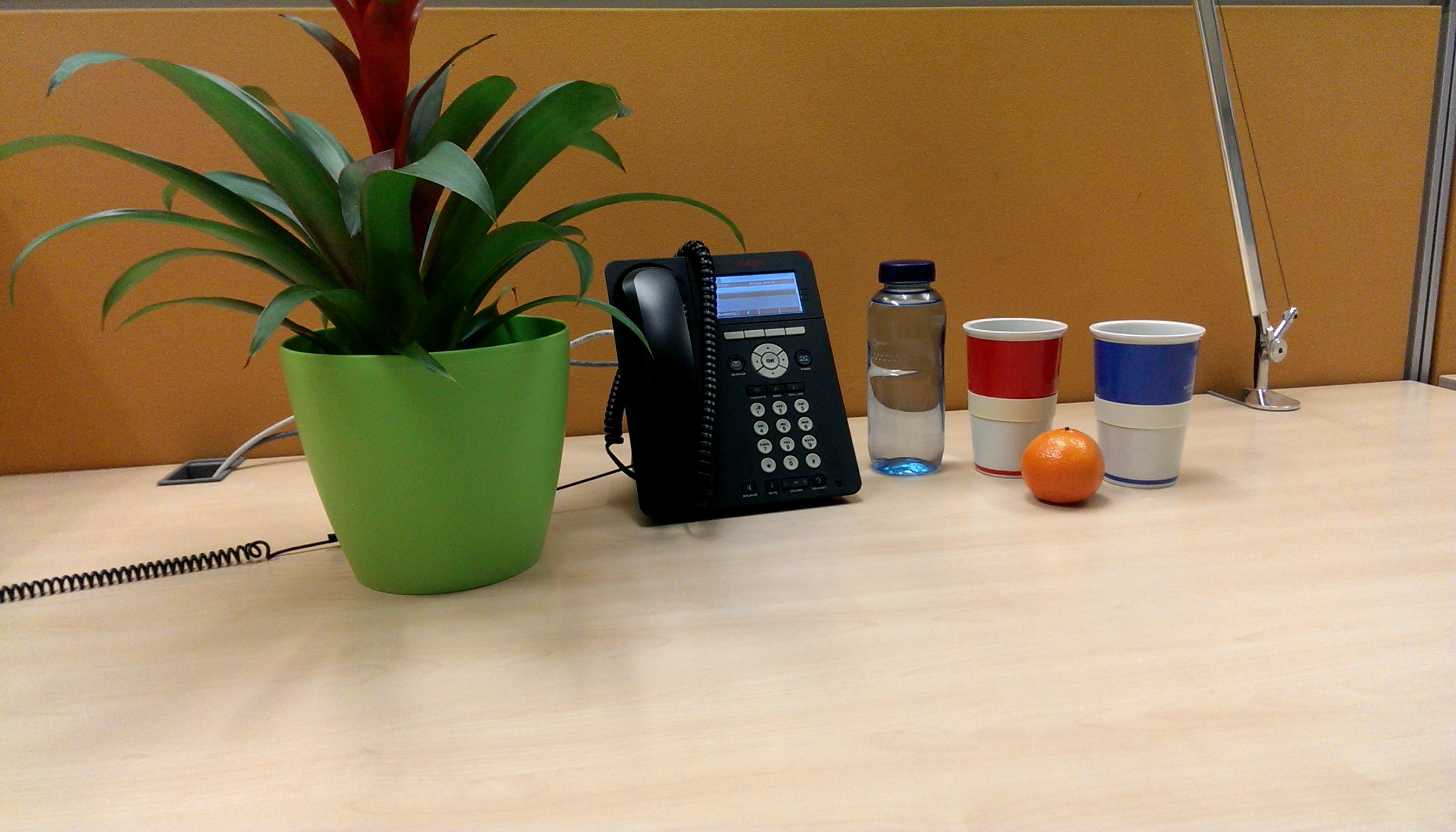
\includegraphics[width=1.4\textwidth]{img/Fotos/QuantiPic_Original.png}
	\caption[QuantiPic Originalbild]{QuantiPic im Originalbild-Modus}
	\label{fig:quanti_orig}
\end{figure}

\begin{figure}[h]
	\centering
		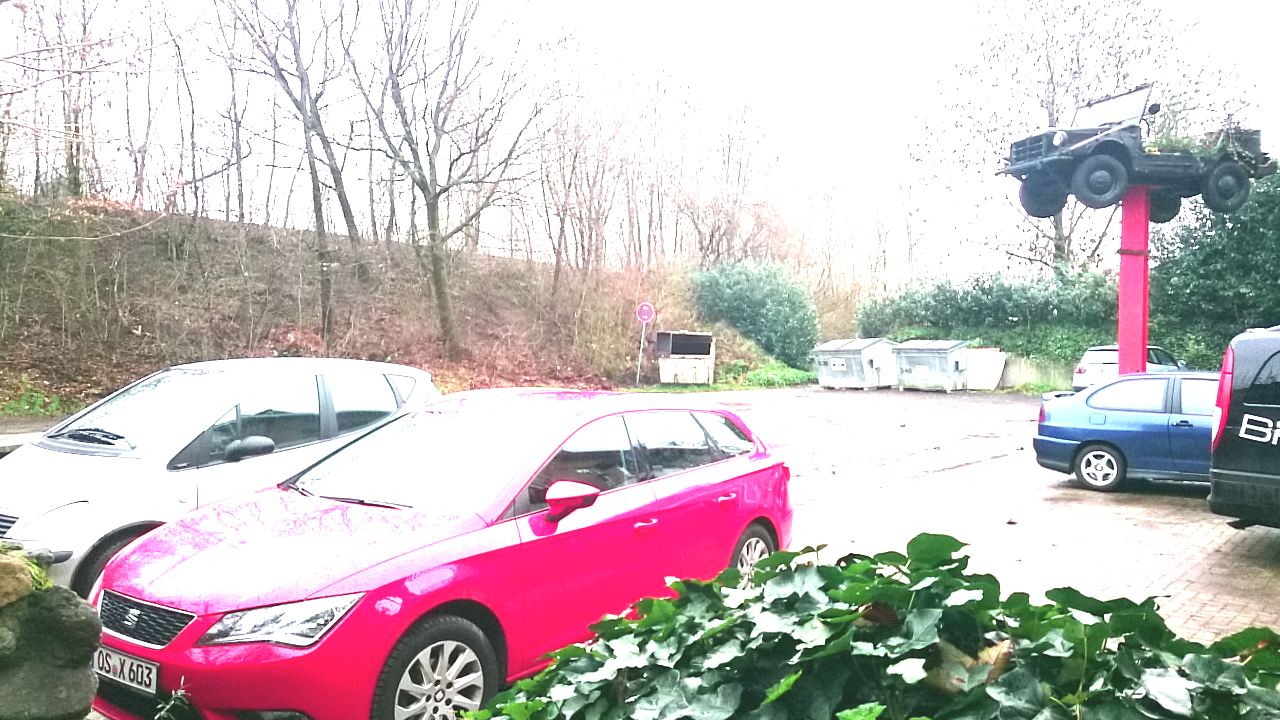
\includegraphics[width=1.4\textwidth]{img/Fotos/QuantiPic_Helligkeit.png}
	\caption[QuantiPic Helligkeit]{QuantiPic im Helligkeits-Modus}
	\label{fig:quanti_hell}
\end{figure}

\begin{figure}[h]
	\centering
		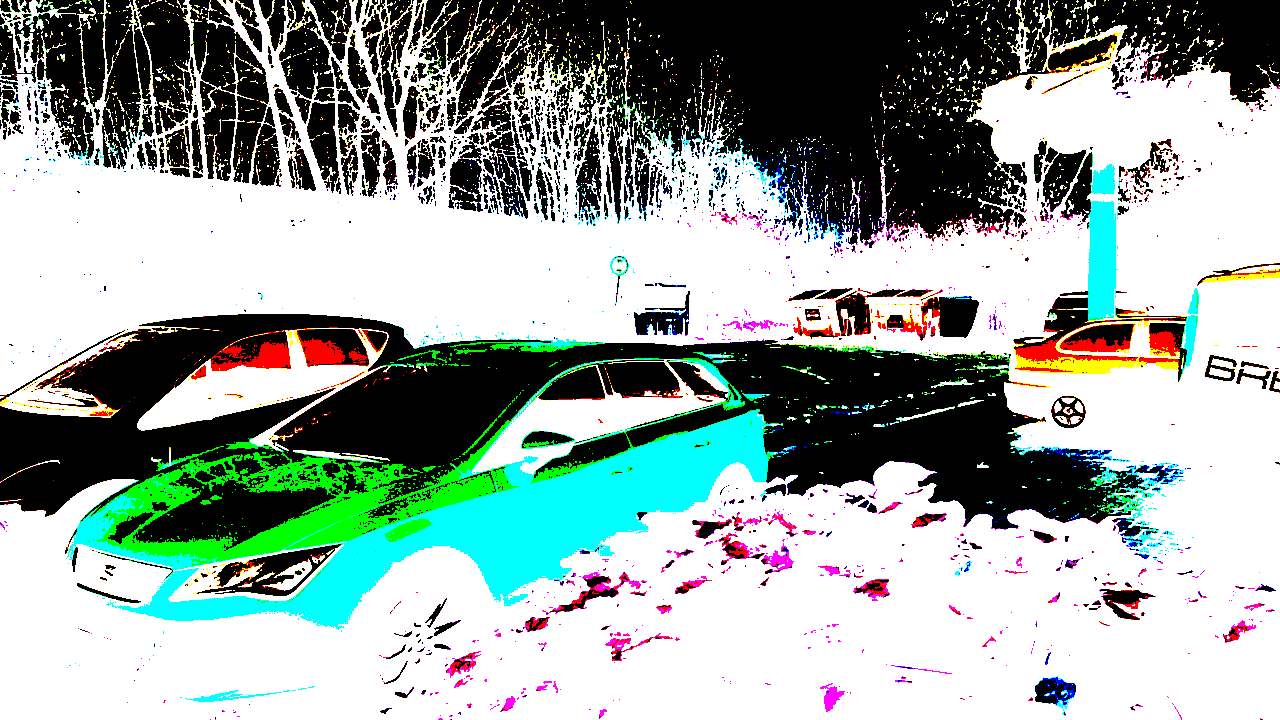
\includegraphics[width=1.4\textwidth]{img/Fotos/QuantiPic_Farbwerte.png}
	\caption[QuantiPic Farbwerte]{QuantiPic im Farbwerts-Modus}
	\label{fig:quanti_farb}
\end{figure}





\end{landscape} 

\subsection{\textbf{Produkteinsatz}}

\subsubsection{Anwendungsbereiche}
Aktuell soll die APP nur für die Studenten der \acs{HfTL} zugänglich sein, welche ein Android-Smartphone besitzen. 

\subsubsection{Zielgruppen, Qualifikationsniveau}

Da bei der Nutzergruppe von Studenten mit Erfahrung im Umgang mit solchen APP's ausgegangen werden kann, wird auch die Oberfläche dementsprechend gestaltet.

\subsection{\textbf{Produktfunktionalität}}

Auszug aus der Aufgabenbeschreibung:

\textit{"Auf Basis der Analyse ist eine neue App zu programmieren,
welch die positiven Eigenschaften der vorhandenen Apps vereint und als Verarbeitungsfunktion
das Bild gleichmäßig mit einem einstellbaren Quantisierungsintervall quantisiert."} 

\subsection{\textbf{Randbedingungen}}

Der zeitliche Rahmen für die Entwicklung und Programmierung dieser APP endet mit der 4. Kalenderwoche 2016.

Durch das Projektteam wird es nach Ende des Projektes keine weitere Softwarebetreuung, Wartung oder der gleichen geben. Es finden ebenfalls keine Schulungen oder Einweisungen statt.

\subsection{\textbf{Annahmen und Abhängigkeiten}}

Die APP wird für Android-Geräte ab Version 4.0.3 zur Verfügung gestellt.
Entsprechend der Vorgaben der Deutschen Telekom AG muss bei der Programmierung der APP, explizit beim Design, auf die Konzernrichtlinien geachtet werden. Es soll zusätzlich auf die Designempfehlungen für Androidgeräte geachtet werden.

%\subsection{\textbf{Verzögerungen}}
%
%Durch die strikte Abtrennung des zeitlichen Rahmens auf das \acs{SoSe15} darf es über diesen Zeitraum hinaus nicht zu Verzögerungen kommen

%\section{Anwendungsszenarien}
%
%\subsection{\textbf{Beschreibung aus der Nutzersicht}}
%
%Die Benutzeroberfläche muss intuitiv bedienbar sein. Der strukturierte Aufbau durch Kategorien (News, Noten, Stundenplan) soll die Übersichtlichkeit erhöhen.
%Die Logindaten werden verschlüsselt auf dem Smartphone gespeichert und auch verschlüsselt übertragen.
%Durch eine durchgehende und vollständige Dokumentation soll eine Wartung auch durch spätere Matrikel oder Administratoren der Hochschule möglich sein.
%Eine Implementierung weiterer Funktionen soll auch im Nachhinein möglich sein.

\section{Anforderungen}

\subsection{\textbf{Fachkonzept}}
Die \acs{QuantiPig}-APP  wird in Java programmiert, um durch Verwendung bestehender Klassen die Erweiterbarkeit und Realisierbarkeit zu vereinfachen. Für das Design werden \acs{XML}-Stylesheets verwendet.


%\subsubsection{Überblick über das Gesamtsystem}
%$\;$ \\ %Zeilenumbruch bei Nutzung von paragraph
%
%\textbf{Noten}
%\begin{itemize}
%	\item die APP soll die Noten lokal auf dem Smartphone nach Semester geordnet anzeigen
%	\item Login im \acs{QIS}-System durch die APP
%	\item Anmeldung über gesicherte, verschlüsselte Übertragung (\acs{HTTPS})
%	\item verschlüsselte Speicherung der Daten auf dem Smartphone (\acs{AES})
%	\item Pull-Nachrichten (Einstellbares Intervall und/oder manuell)
%	\item Benachrichtigung bei Eingang von neuen Noten
%	\item Nutzer wird mit Hinweismeldungen informiert, wenn Noten aktualisiert wurden
%\end{itemize}
%Optionale Angaben im Menüpunkt Noten:
%\begin{itemize}
%	\item Klassenspiegel
%	\item Notenverteilung
%	\item Anzahl der Teilnehmer
%	\item Notenschnitt
%	\item Anzeige der Creditpoints
%	\item zu erreichende Creditpoints
%	\item erreichte Creditpoints
%\end{itemize}
%\textbf{Stundenpläne}
%\begin{itemize}
%	\item Stundenplan nur für zum Nutzer passenden Studiengang
%	\item Pull-Nachrichten (Einstellbares Intervall und/oder manuelle Abfrage)
%	\item Synchronisierung mit dem Kalender auf dem Smartphone	
%\end{itemize}
%\textbf{News}
%\begin{itemize}
%	\item Pull-Nachrichten (manuelle Aktualisierung)
%	\item News von: \url{https://www.hft-leipzig.de/de/studierende/service/news.html}
%\end{itemize}



\subsubsection{Verwendete Bibliotheken von Drittanbieteren}
\begin{itemize}
	\item OpenCV 
\end{itemize}


%\subsection{\textbf{Anforderungen an die Datenhaltung}}
%
%Alle gespeicherten Daten müssen vor unbefugtem Zugriff geschützt werden, dafür werden Benutzerdaten in einer \acs{SQL}-Datenbank gespeichert. Die Datenbank darf nur durch die App abgefragt werden. Passwort und Benutzername werden mit \acs{AES} verschlüsselt.

%\subsubsection{allgemeine Beschreibung der Daten}
%Sicherheitsrelevante Daten sind in dem Notenteil der App zu finden. Diese sind der Benutzername, das Passwort, die Prüfungs- und Prüfungsvorleistungsergebnisse, der Klassenspiegel und die Creditpoints.
%Die öffentlichen Daten sind in den anderen beiden Teilen der App enthalten.
%Dazu gehören die News mit ihren Terminen und Inhalt und die Stundenpläne mit den Veranstaltungen und den dazugehörenden Informationen wie Dozent und Veranstaltungsort.


%\subsection{\textbf{Anforderungen an die Benutzeroberfläche}}
%
%\subsubsection{allgemeine Anforderungen an die Oberfläche}
%
%Das Layout richtet sich nach dem  \ac{CI/CD} der Deutschen Telekom AG, speziell dem der \acs{HfTL} Trägergesellschaft, stand 14.12.12. Entsprechend sind primär die Farben, sowie Schriftarten vorgegeben. Das Layout zieht sich einheitlich (mit funktionsbedingten Abweichungen) durch alle APP-Teile und soll eine leichte Bedienung begünstigen.
%Die Größe der einzelnen Elemente (Buttons, Zeilen, Überschriften etc.) ist an den Designempfehlungen seitens Android angelehnt. 
%Auch die Abstände zwischen den einzelnen Elementen wurden – sofern sie mit dem \ac{CI/CD} in Einklang stehen – entsprechend der Designempfehlung festgelegt.
%Die Reaktionszeit der Benutzereingaben soll mit möglichst geringer Verzögerung verarbeitet und dargestellt werden.






%\subsubsection{Berechtigungen}
%
%Die APP wird als Open Source bereitgestellt.
%
%Nicht angemeldete Benutzer können sich die News und die Stundenpläne anzeigen lassen. Angemeldete Benutzer können zusätzlich ihre Noten abrufen.
%
%Die App braucht folgende Berechtigung auf dem Smartphone:
%\begin{itemize}
%	\item Netzwerkstatus abrufen: zur Kontrolle ob das Handy online ist
%	\item Internet: APP greift auf das Internet zu
%	\item Telefonstatus: wird zur Verschlüsselung benötigt
%	\item Kalendereintäge bearbeiten
%	\item darf beim Systemstart ausgeführt werden
%\end{itemize}




%\subsubsection{Bildschirmlayout}
%siehe Anhang \ref{subsec:App-Layout}





%\subsubsection{Dialogstruktur, Dialogabläufe}
%\textcolor{magenta}{Maik/Stefan bitte hier Screenshots der jeweiligen %Dialoge einfügen oder in Anhang unter Dialogmasken}





%\subsection{\textbf{Leistungsanforderungen}}
%Es wird von einer maximalen Nutzerzahl von 1000 Studenten ausgegangen.
%Die Reaktionszeit/Programmstart der APP soll möglichst gering gehalten werden.
%Das Datenaufkommen soll möglichst gering ausfallen.


\subsection{\textbf{Anfordeungen für Inbetriebnahme und Einsatz}}

%\subsubsection{Sicherheitsziele}
%Der Benutzername und das Passwort werden in einem gesicherten Speicherbereich (nur root), mit \acs{AES} verschlüsselt, gespeichert.
%Die Datenbank in der die Noten gespeichert werden, liegt ebenfalls in diesem Bereich und darf nur von der \acs{HfTL}-App geöffnet werden.
%Die Kommunikation mit der \acs{HfTL}-Webseite und \acs{QIS} erfolgt gesichert per \acs{HTTPS}.



\subsubsection{Installationsprozedur}

Die \acs{APP} wird als .apk Datei ausgeliefert und kann somit manuel auf Android-Smartphones ab Version 4.4.2 installiert werden.
Dabei muss das Installieren von Software mit unbekannter Herkunft erlaubt werden.


%\subsubsection{Pilot- bzw. Probebetrieb}
%
%siehe Anhang Versionsmanagementprotokolle \ref{subsec:Release-Historie}





%\subsubsection{Fehlerreaktion, Garantie, Service, »Wiederanlauf«}
%Die Zuverlässigkeit sollte sich durch eine große \ac{MTBF} darstellen.



%\subsubsection{Schulungen}
%Nach Beendigung des Projektes werden keine Schulungen usw. durchgeführt.


\subsection{\textbf{Qualitätsanforderungen}}

\subsubsection{Qualitätsmerkmale}
Folgende Qualitätsansprüche werden gestellt:
\begin{itemize}
	\item Hohe Zuverlässigkeit der Software
	\item schnelle und zuverlässige Verarbeitung der gewünschten Daten
	\item Fehler werden mit einer entsprechenden Fehlermeldung beantwortet
	\item Intuitiv benutzbar
	\item Leicht zu warten und zu erweitern
	\item Vollständige Dokumentation des Projektes
\end{itemize}




%\subsubsection{Qualitätssicherung}
%Zur Qualitätssicherung werden einheitliche Testprotokolle und die entsprechenden Testkriterien erstellt. Es finden regelmäßige Kontrollen durch die Qualitätssicherung statt, um die Einhaltung der gegebenen Standards zu überprüfen. Es findet ebenfalls eine regelmäßige Kontrolle der Dokumentation statt. Die jeweiligen Software-Prototypen werden nach der Prototypisierung zur Fehlererkennung und zum Funktionstest an das Projektteam geschickt. Zur Verbesserung der Software werden die Tests anhand vorgegebener Testkriterien durchgeführt, um standardisierte Testergebnisse zu erhalten. Die Testergebnisse werden zur Auswertung an die entsprechende Projektgruppen zurück gespiegelt.


%\subsubsection{Qualitätsnachweise}
%Während des Projektzeitraumes werden sämtliche Meeting, Tests und Kontrollen protokolliert und zur Dokumentation in einem dafür vorgesehen Bereich abgelegt. Die gesetzten Standards und Vorgaben werden eingehalten. Zum Projektabschluss ist der geplante Umfang erreicht und alle Muss-Kriterien sind enthalten. Die APP ist funktionstüchtig.



%\subsubsection{Offenlegung der Qualitätskontrollpläne}
%
%\begin{tabular}{lll}
%	\textbf{Nr.} & \textbf{Anforderung} & \textbf{Verantwortliche} \\
%	1 & Projektrahmen festlegen & gesamtes Team \\
%	1.1 & Projektrahmen festlegen & gesamtes Team \\
%	1.2 & Architektur & gesamtes Team \\
%	1.3 & Vorgehensmodell & gesamtes Team \\
%	\\
%	2 & Vollständige Dokumentation & gesamtes Team \\
%	2.1 & UML Diagramme erstellen & AD, CM \\
%	2.2 & Installationsanleitung und Benutzerhandbuch erstellen & GE, JS \\
%	2.3 & Lasten- Pflichtenheft erstellen & SK, SC \\
%	2.4 & Protokolle & ML, PK \\
%	2.5 & Dokumentation zusammenstellen und gestalten & JS, SC \\
%	\\
%	3 & App erstellen & gesamtes Team \\
%	3.1 & Design nach HfTL-Vorgaben erstellen & ML, SC \\
%	3.2 & Programmierung der APP & GE \\	
%	\\
%	4 & Qualitätskontrolle & gesamtes Team \\
%	4.1 & Testkriterien festlegen & PK \\
%	4.2 & Testprotokollelayout erstellen & ML \\
%	4.3 & Softwaretests & ML, PK \\
%	4.4 & Kontrolle der Dokumentation & PK \\
%	\\
%	5 & Anfertigen der Präsentation & gesamte Team \\
%	5.1 & Präsentation halten & SC, ML, SK, JS \\
%\end{tabular}



%\subsubsection{Berichte, Protokolle zum Nachweis des Vorgehens gemäß der Qualitätskontrollpläne}
%
%siehe Anhang "'Testprotokolle"' \ref{subsec:Testprotokolle}
%und Anhang "'Sitzungsprotokolle"' \ref{subsec:Sitzungsprotokolle}



\subsection{\textbf{Anforderung an die Entwicklung}}

\subsubsection{Entwicklungs-Umgebung}
Für die Entwicklung wird Android Studio inkl. Gradle in der Version 1.x genutzt. Für die Dokumentation und Projektkoordination wird GitHub verwendet.
Die Dokumentation wird mittels \LaTeX{} erstellt.



%\subsubsection{Projekt-Organisation}
%Die Projektorganisation wird wie in folgender Abbildung strukturiert. Als Vorgehensmodell wird das Spiralmodell mit Prototyping gewählt. Es ist ein iteratives Modell, wobei jeder Zyklus in den einzelnen Quadranten folgende Aktivitäten enthält:
%
%\begin{itemize}
%	\item Festlegung von Zielen, Identifikation von Alternativen und Beschreibung von Rahmenbedingungen
%	\item Evaluierung der Alternativen und das Erkennen, Abschätzen und Reduzieren von Risiken, z. B. durch Analysen, Simulationen oder Prototyping
%	\item Realisierung und Überprüfung des Zwischenprodukts
%	\item Planung des nächsten Zyklus der Projektfortsetzung.
%\end{itemize}
%
%Die einzelnen Aufgaben werden Personen zugeordnet. In wöchentlichen Online-Meetings über Teamviewer stellt jeder seine Ergebnisse vor und es werden diese bewertet. Anhand dieser Ergebnisse werden für den neuen Zyklus Aufgaben verteilt. Der Protokollführer hält alle Ergebnisse und Aufgaben fest und legt die Protokolle im Projektordner ab.
%
%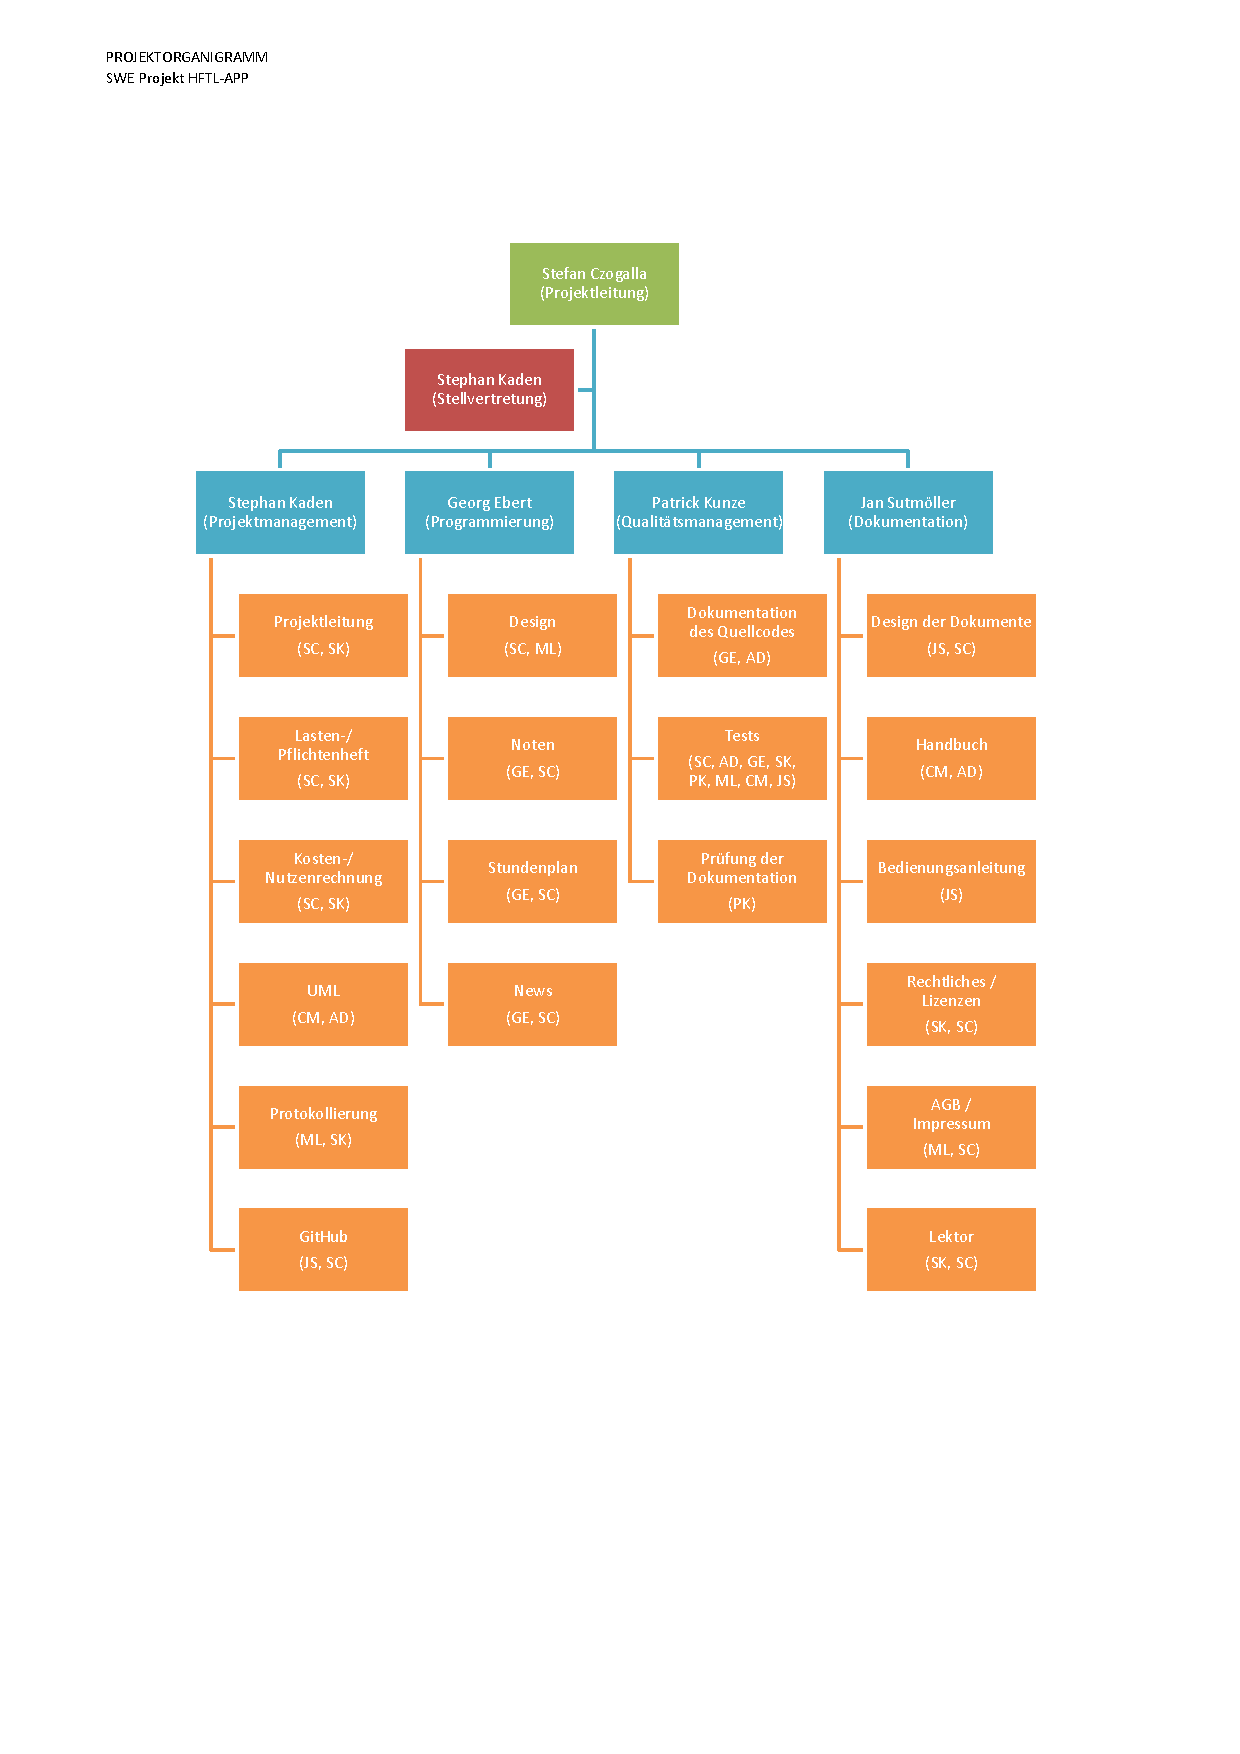
\includepdf[pages=-,noautoscale]{04_Anhang/files/swe_organigramm2.pdf}
%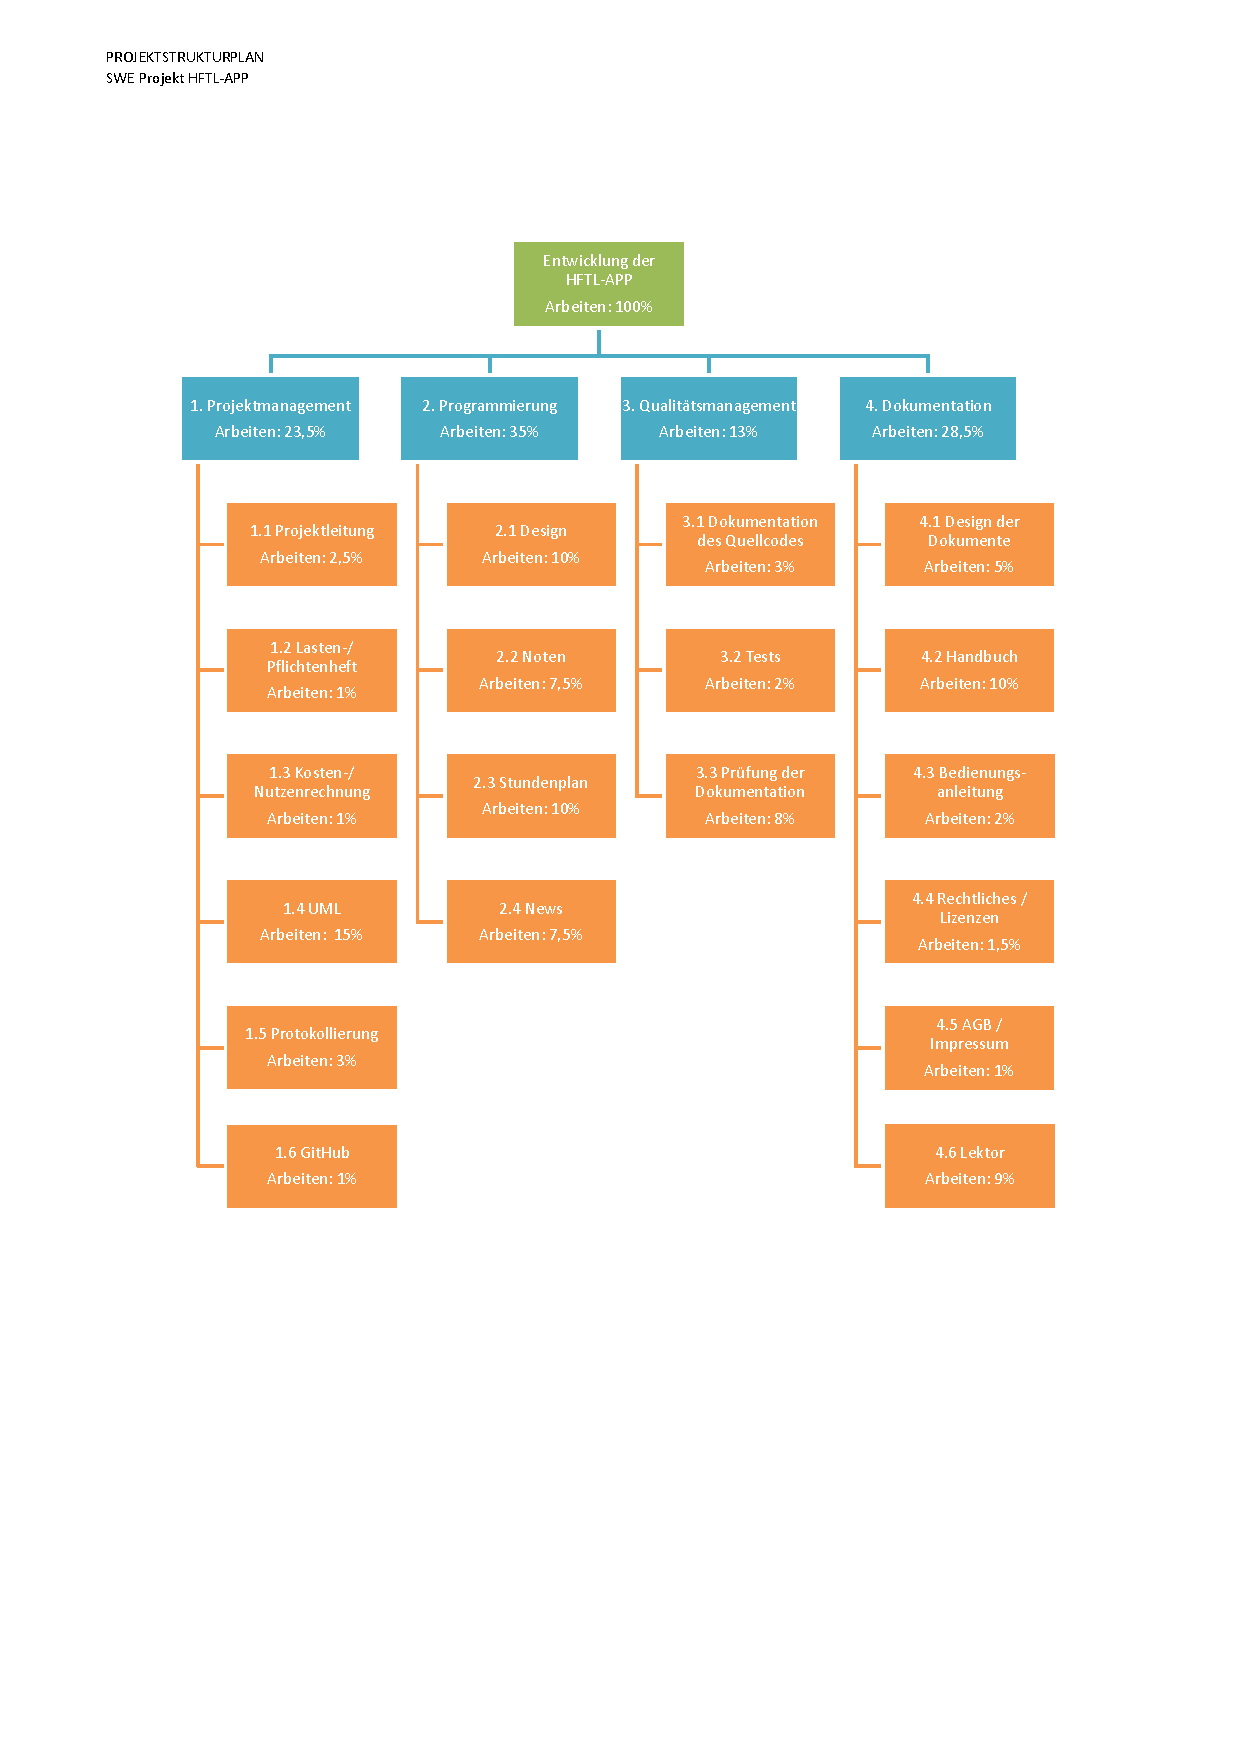
\includepdf[pages=-,noautoscale]{04_Anhang/files/swe_projektstrukturplan.pdf}


%\subsubsection{Projekt-Planung}
%siehe Anhang "'Gantt"' \ref{subsec:Gantt}

\subsubsection{Änderungsmanagement}
Zur Versionsverwaltung wurde Git eingesetzt. Als Hosting-Anbieter wurde dabei auf GitHub gesetzt, welcher einen kostenfreien Zugang für nicht kommerzielle Projekte bereitstellt. Ein \ac{GUI} oder ein Konsolenprogramm für Windows und Linux übernehmen dabei die Steuerung der Versionsverwaltung. Konflikte in den einzelnen Versionen können nur über die Konsole behoben werden. Auf der Webseite von GitHub können Milestones erstellt werden und an die jeweiligen Mitarbeiter zugeteilt werden. In den Milestones werden einzelne Aufgaben, sogenannte Issues angelegt und wiederum den Bearbeitern zugeordnet, somit ist der Bearbeitungsstand zu jeder Zeit des Projektes ersichtlich und es kann schnell auf sich ergebende Probleme reagiert werden.



%\subsubsection{Testanforderungen}
%siehe Anhang "'Testprotokollentwurf"' \ref{subsec:Testprotokollentwurf}

\section{Ergebnis}
\subsection{Umfang der APP}
Die App wurde, angelehnt an die Namen der vorhandenen Apps, "QuantiPig" genannt. Als Logo wurde ein Schweinekopf gewählt.
\begin{figure}[h]
	\centering
		
\includegraphics[width=0.4\textwidth]{img/ic_launcher.png}
	\caption[QuantiPig Logo]{QuantiPig Logo}
	\label{fig:pig_logo}
\end{figure}

Als Algorithmen wurde folgende Verfahren implementiert:

\begin{itemize}
	\item keine Quantisierung
	\item skalare Quantisierung mit folgenden Quantisierungsintervallen
		\begin{itemize}
			\item 2x2 px
			\item 4x4 px
			\item 8x8 px
			\item 80x80 px
		\end{itemize}
	\item Midtread-Quantisierung
\end{itemize}


\newpage
\subsection{Erscheinungsbild}
Die APP startet generell im Landscape-Modus. Wie in der folgenden Abbildung zu sehen, gibt es einen jeweils einen Button für die Wahl des Quantisierungsverfahrens und den Auslöser.

\begin{figure}[h]
	\centering
		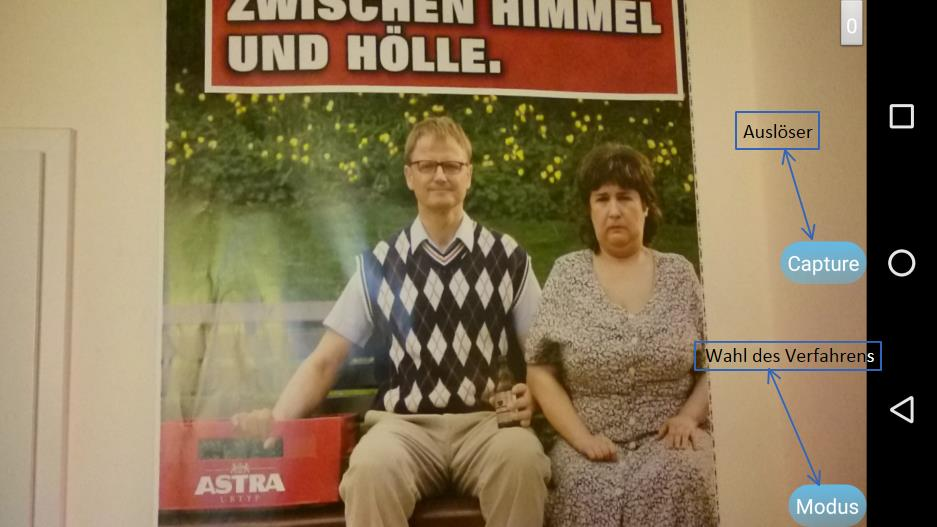
\includegraphics[width=1.0\textwidth]{img/Startbildschirm_QuantiPig.jpg}
	\caption[QuantiPig Startbildschirm]{QuantiPig Startbildschirm}
	\label{fig:pig_menue}
\end{figure}

Nach Drücken auf den Auslöser wird ein Foto mit aktuellem Komprimierungsverfahren gemacht und in den entsprechenden Ordner auf dem Smartphone abgelegt. Als Name wird das jeweilige Verfahren, gefolgt von einem Zeitstempel verwendet.

Nach betätigen des Buttons "Modus", öffnet sich, wie in folgender Abbildung zu sehen, ein Auswahlmenü für die drei verschiedenen Verfahren.

\begin{figure}[h!]
	\centering
		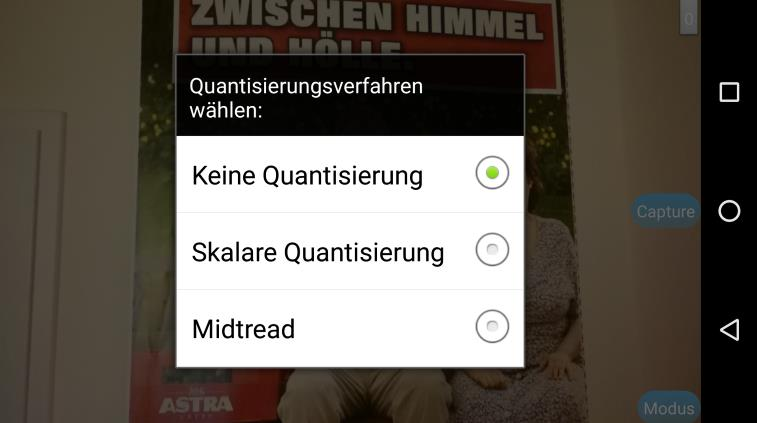
\includegraphics[width=1.0\textwidth]{img/Verfahren_QuantiPig.jpg}
	\caption[QuantiPig-Menü Verarbeitungsverfahren]{QuantiPig-Menü Verarbeitungsverfahren}
	\label{fig:pig_verfahren}
\end{figure}

Im Modus skalare Quantisierung gibt es einen weiteren Button mit dem man das Quantisierungsintervall auswählen kann.

\begin{figure}[h!]
	\centering
		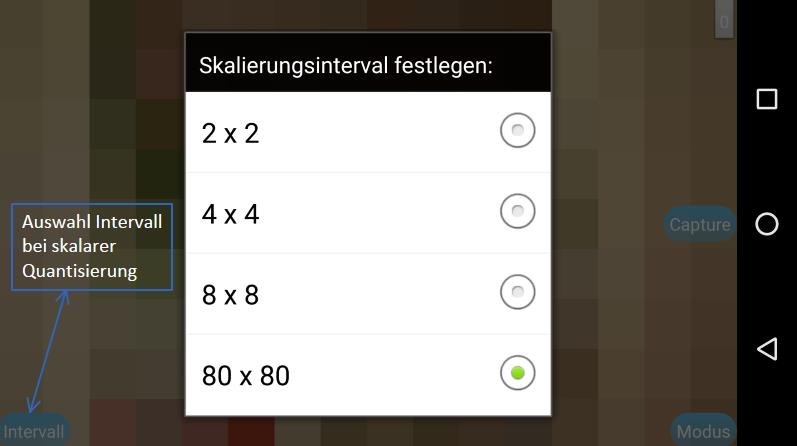
\includegraphics[width=1.0\textwidth]{img/Intervall_QuantiPig.jpg}
	\caption[QuantiPig-Menü Qunatisierungsintervall]{QuantiPig-Menü Qunatisierungsintervall}
	\label{fig:pig_intervall}
\end{figure}

\clearpage



\subsection{Beispielbilder}
\begin{landscape}


\begin{figure}[h]
	\centering
		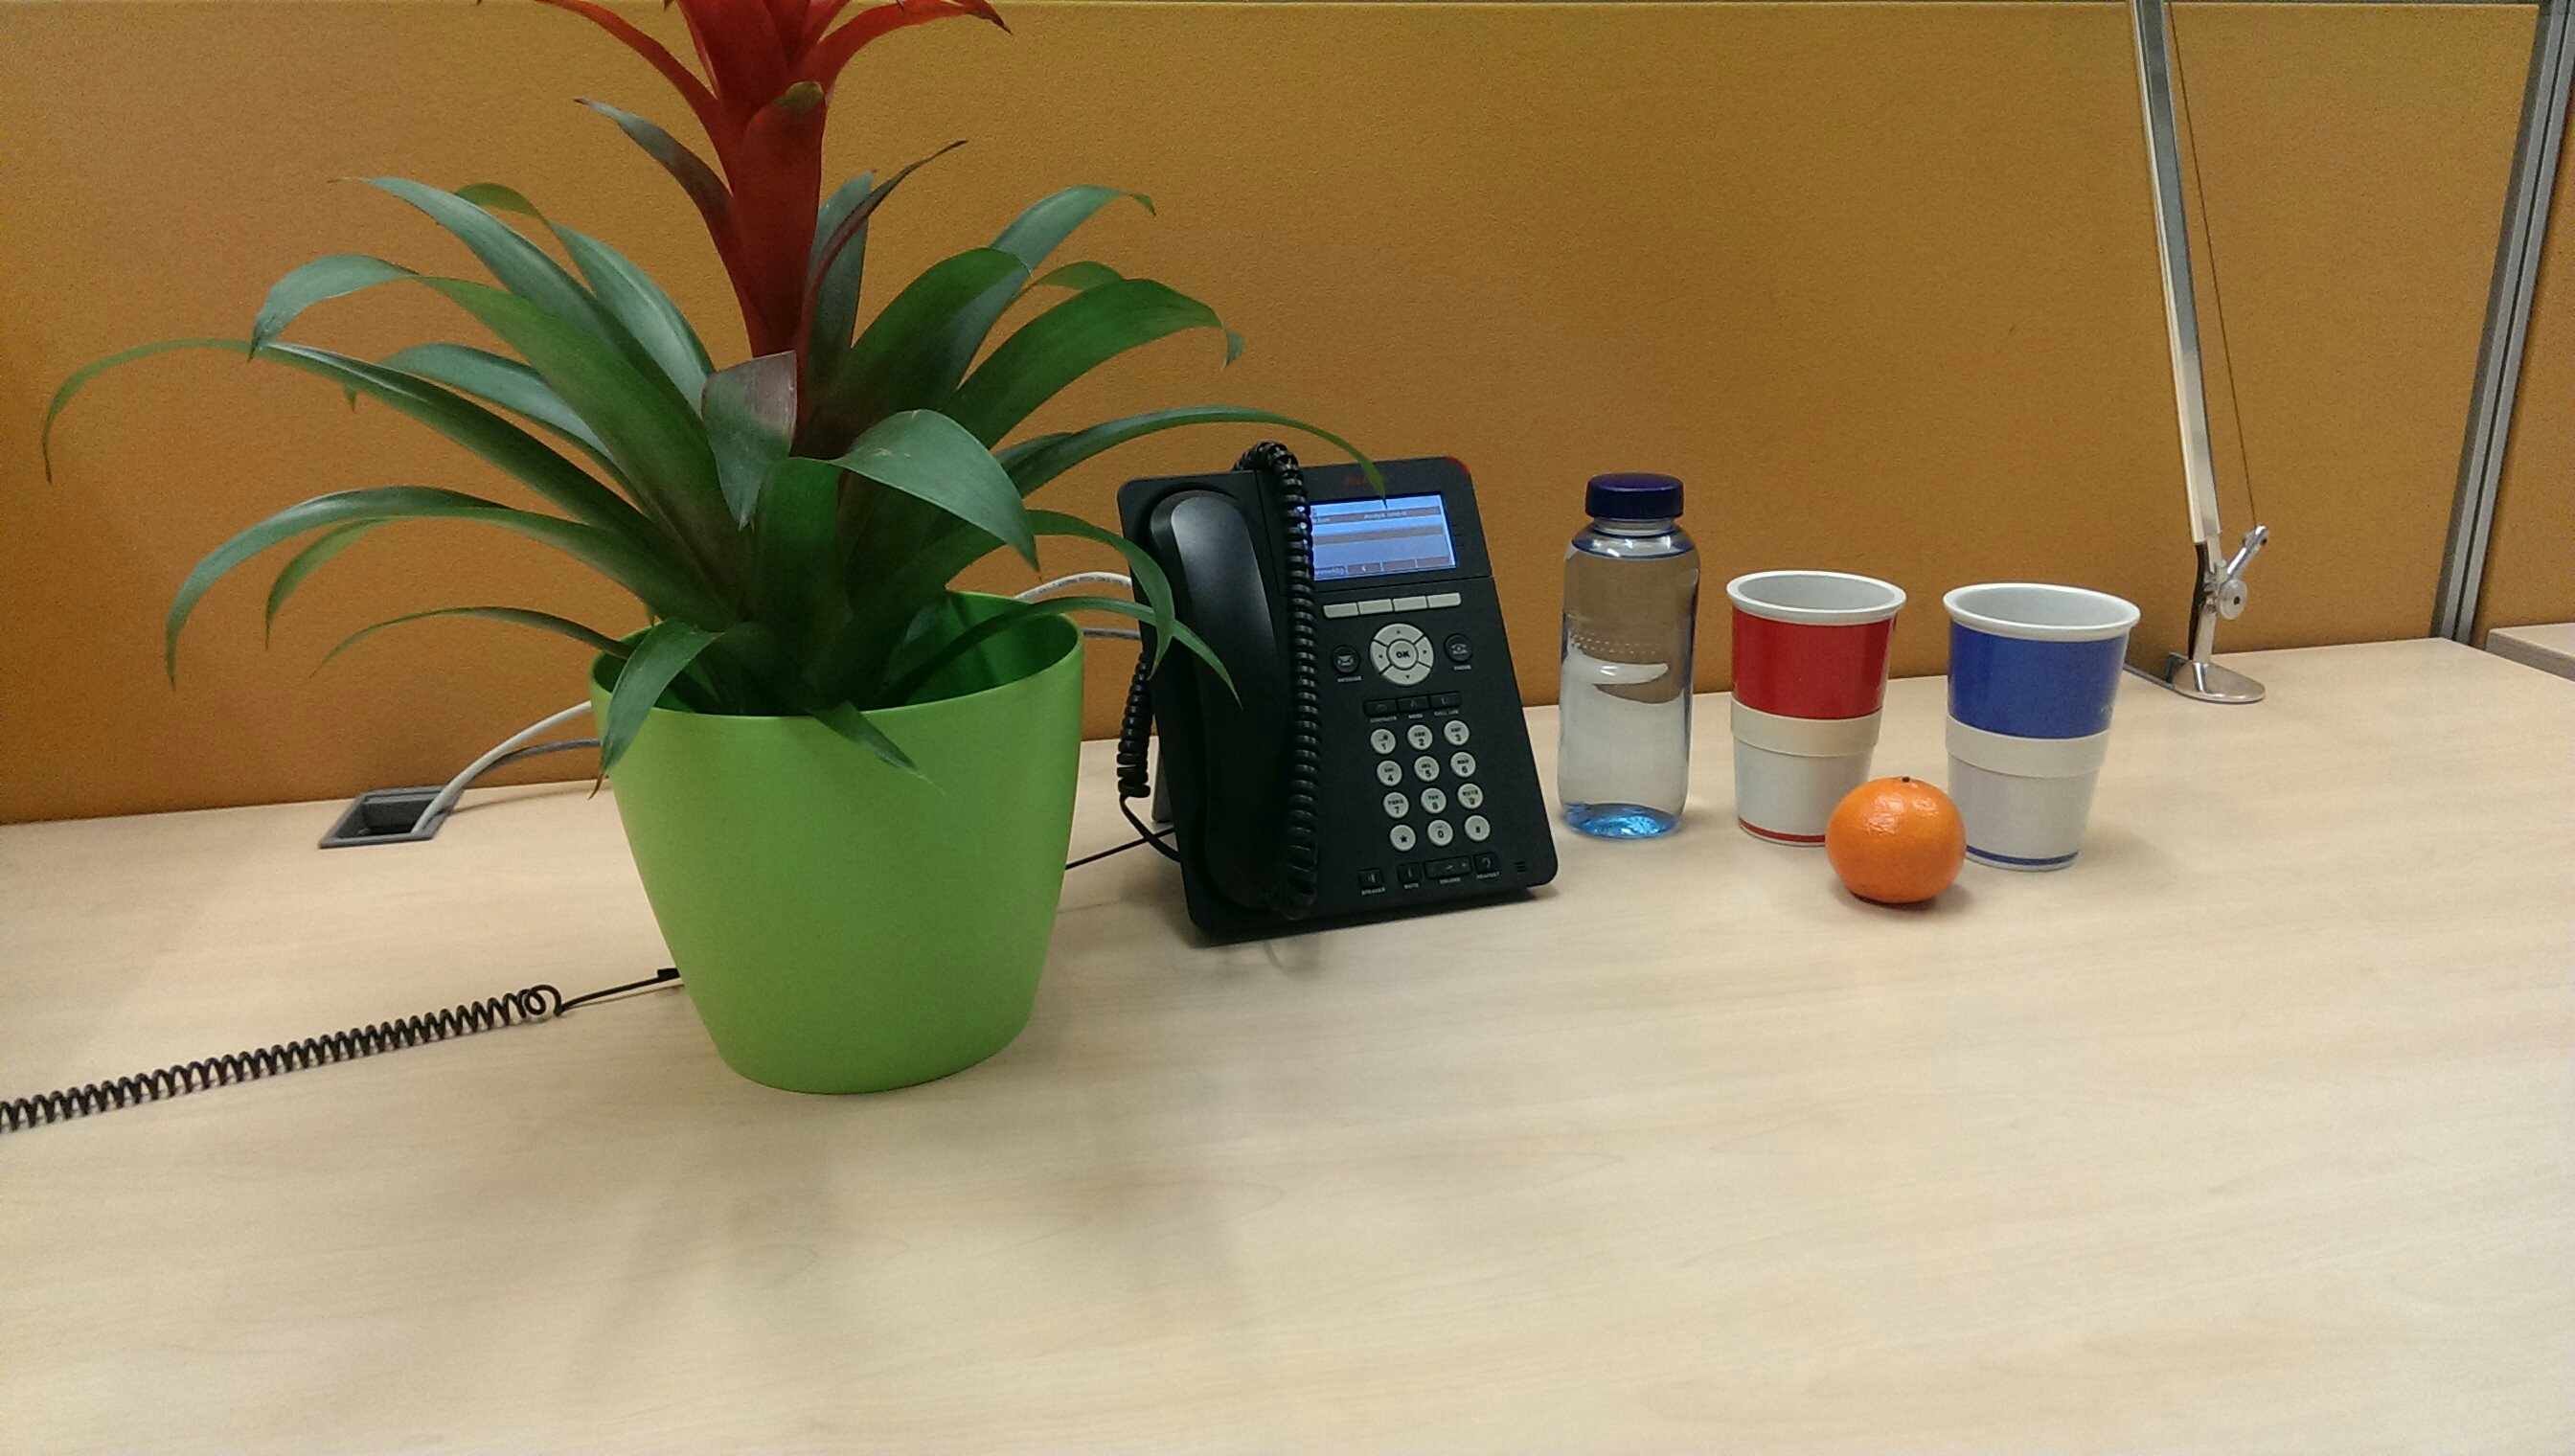
\includegraphics[width=1.4\textwidth]{img/Fotos/QuantiPig_Original.jpg}
	\caption[QuantiPig Originalbild]{QuantiPig Originalbild}
	\label{fig:pig_original}
\end{figure}

\begin{figure}[h]
	\centering
		\includegraphics[width=1.4\textwidth]{img/Fotos/QuantiPig_Midtread.jpg}
	\caption[QuantiPig Midtread]{QuantiPig Midtread}
	\label{fig:pig_midtread}
\end{figure}

\begin{figure}[h]
	\centering
		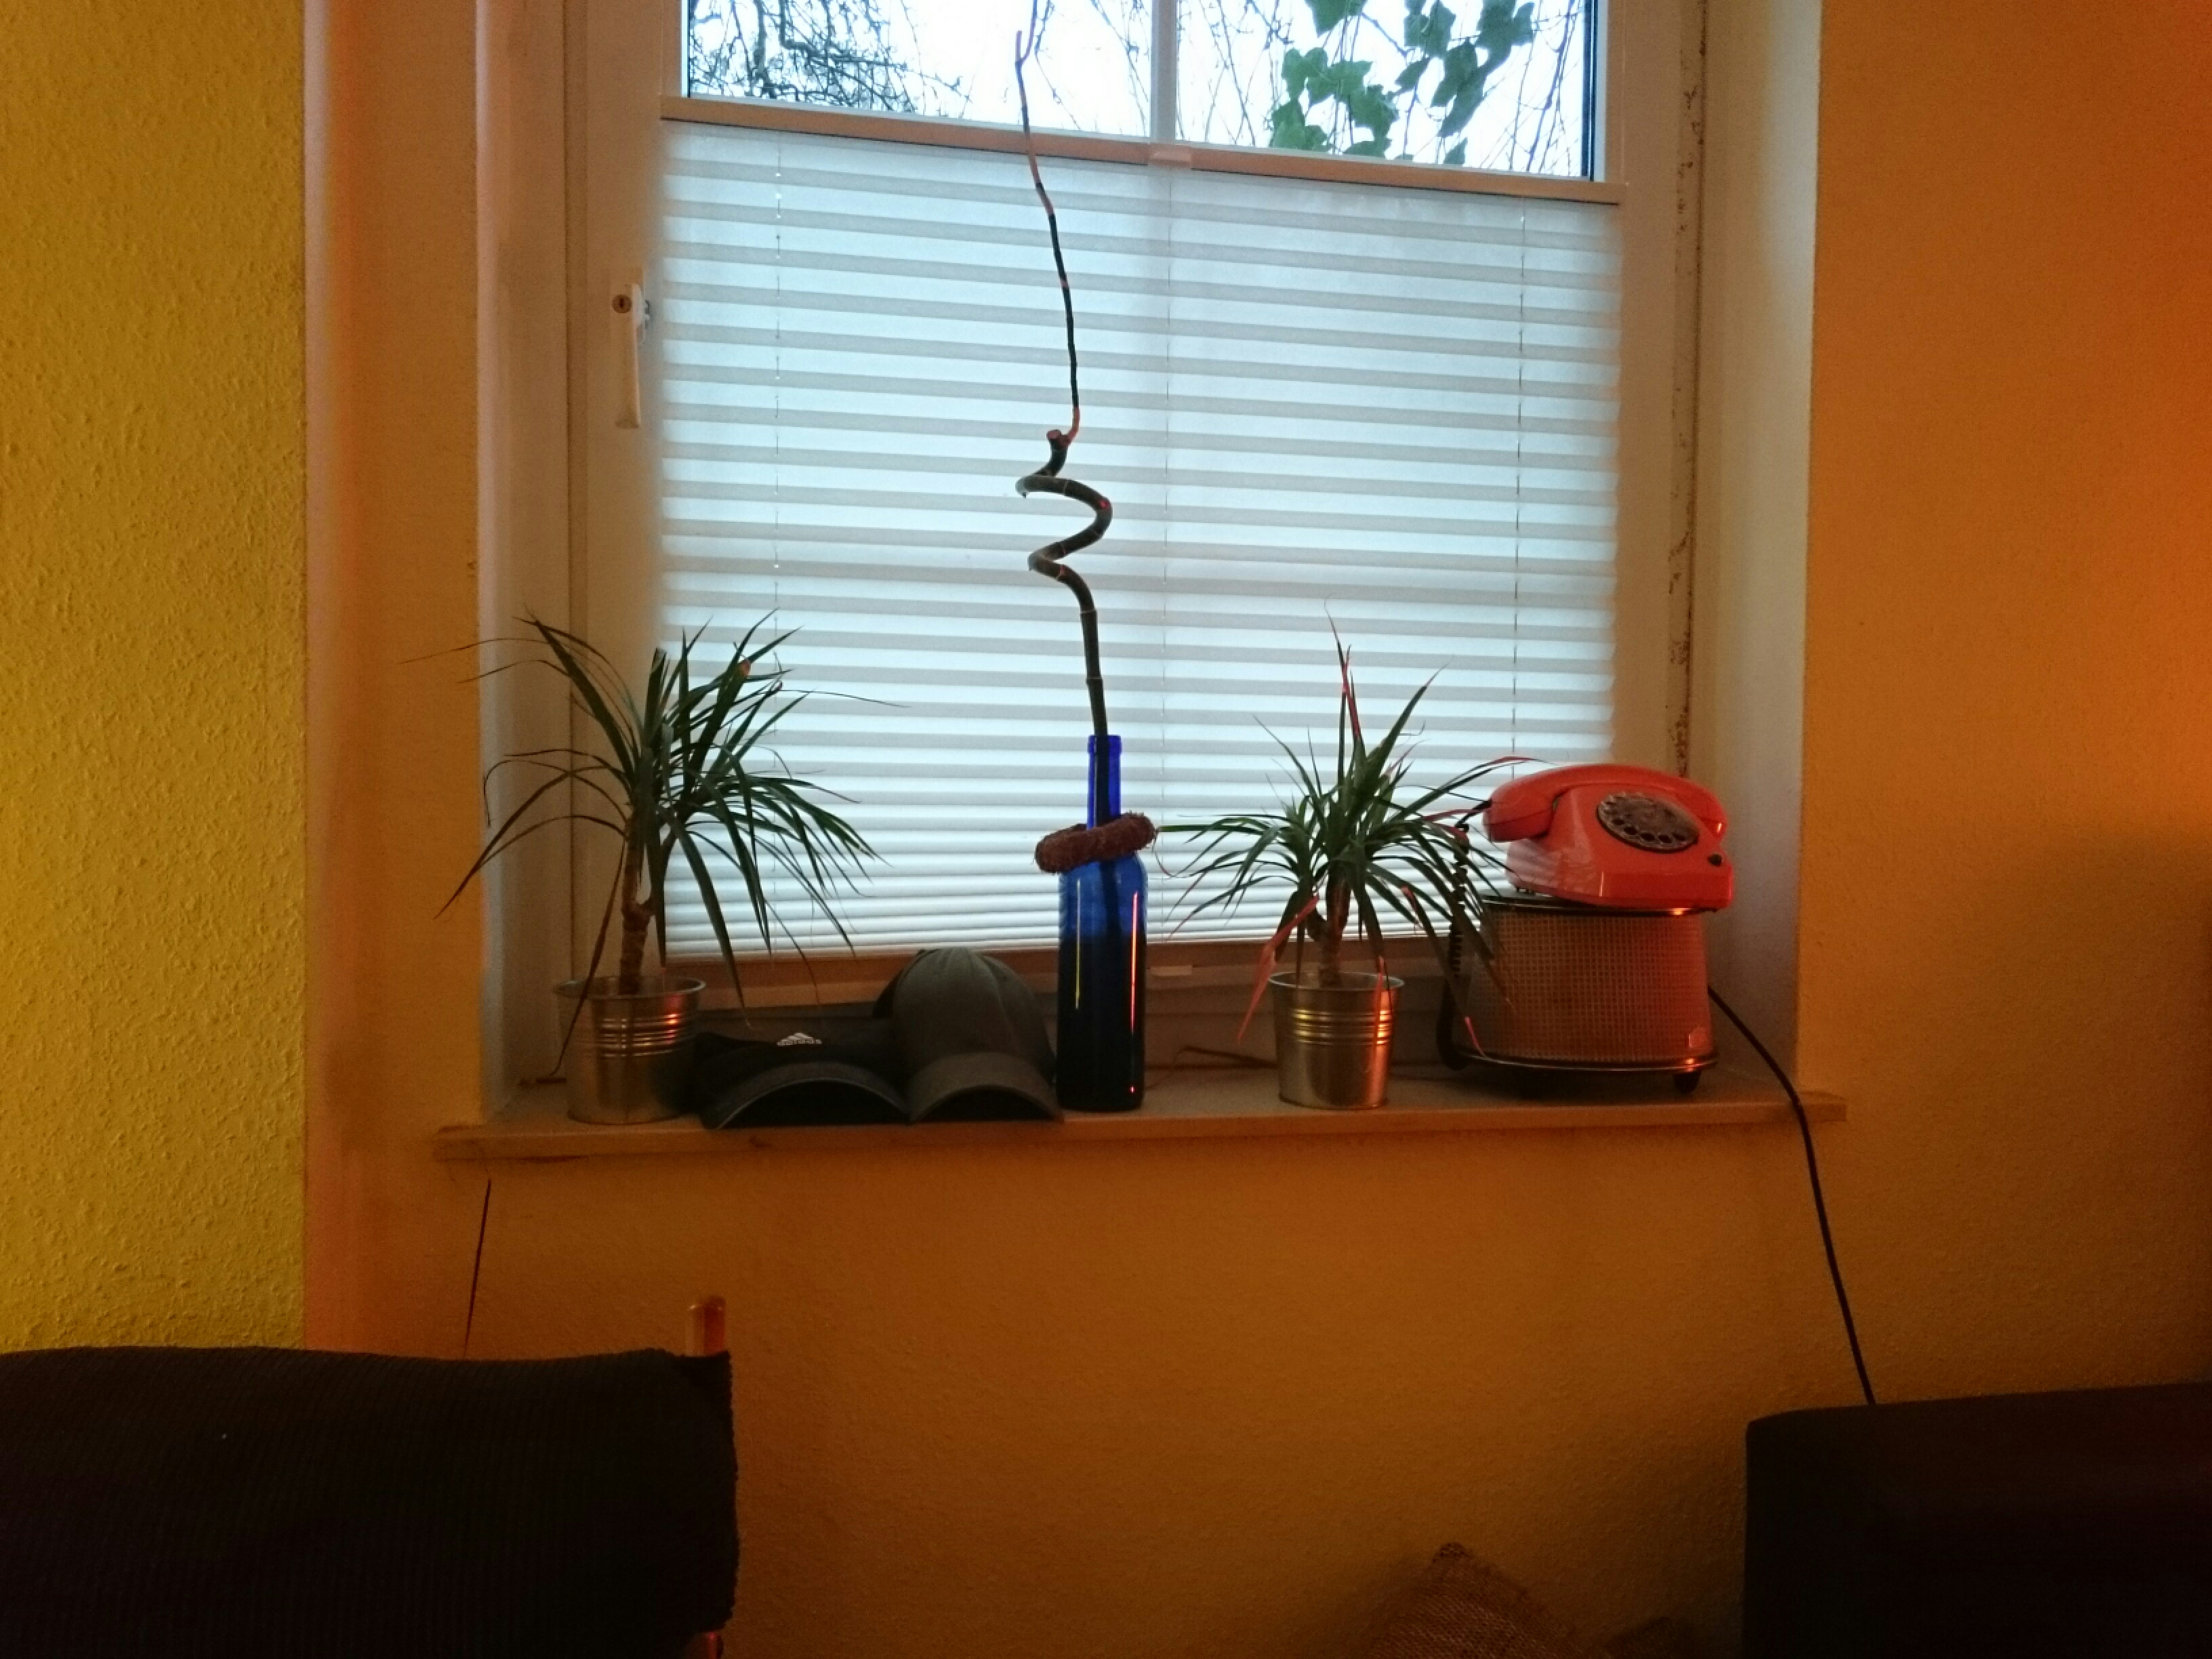
\includegraphics[width=1.4\textwidth]{img/Fotos/QuantiPig_Skalar_2x2.jpg}
	\caption[QuantiPig skalare Quantisierung 2x2 p]{QuantiPig skalare Quantisierung 2x2 px}
	\label{fig:pig_skalar 2x2}
\end{figure}

\begin{figure}[h]
	\centering
		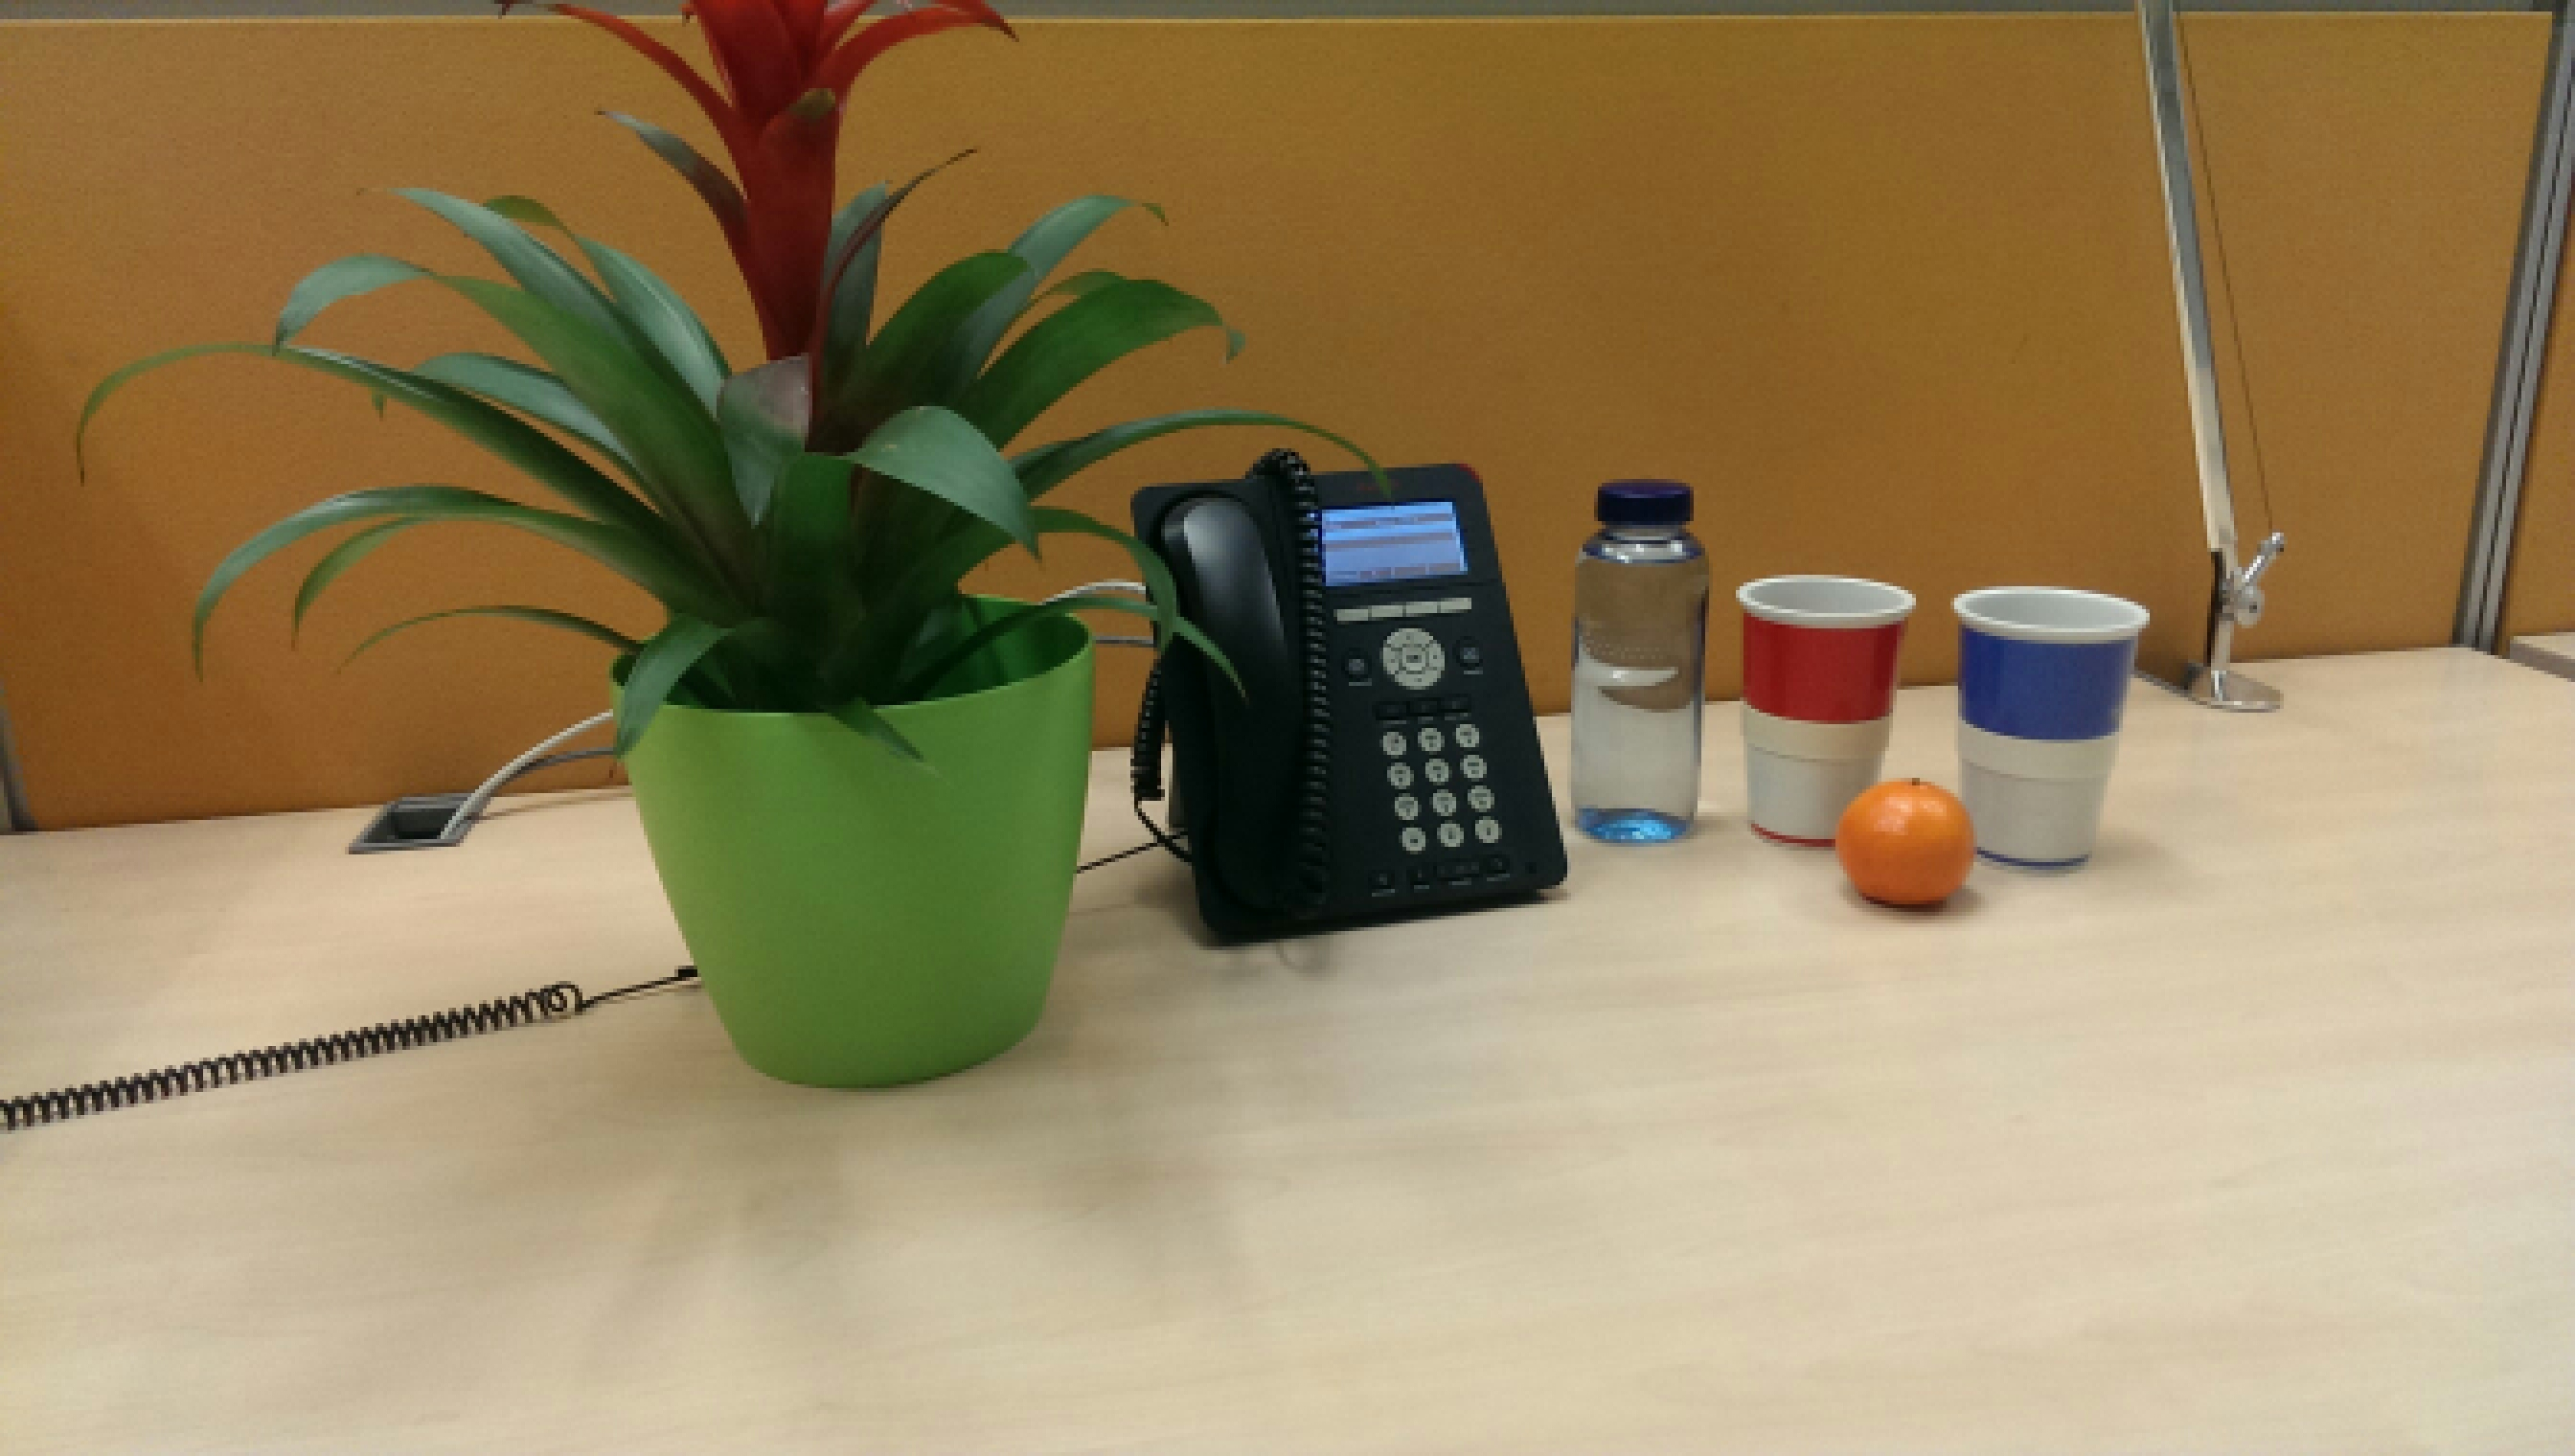
\includegraphics[width=1.4\textwidth]{img/Fotos/QuantiPig_Skalar_4x4.jpg}
	\caption[QuantiPig skalare Quantisierung 4x4 px]{QuantiPig skalare Quantisierung 4x4 px}
	\label{fig:pig_skalar 4x4}
\end{figure}

\begin{figure}[h]
	\centering
		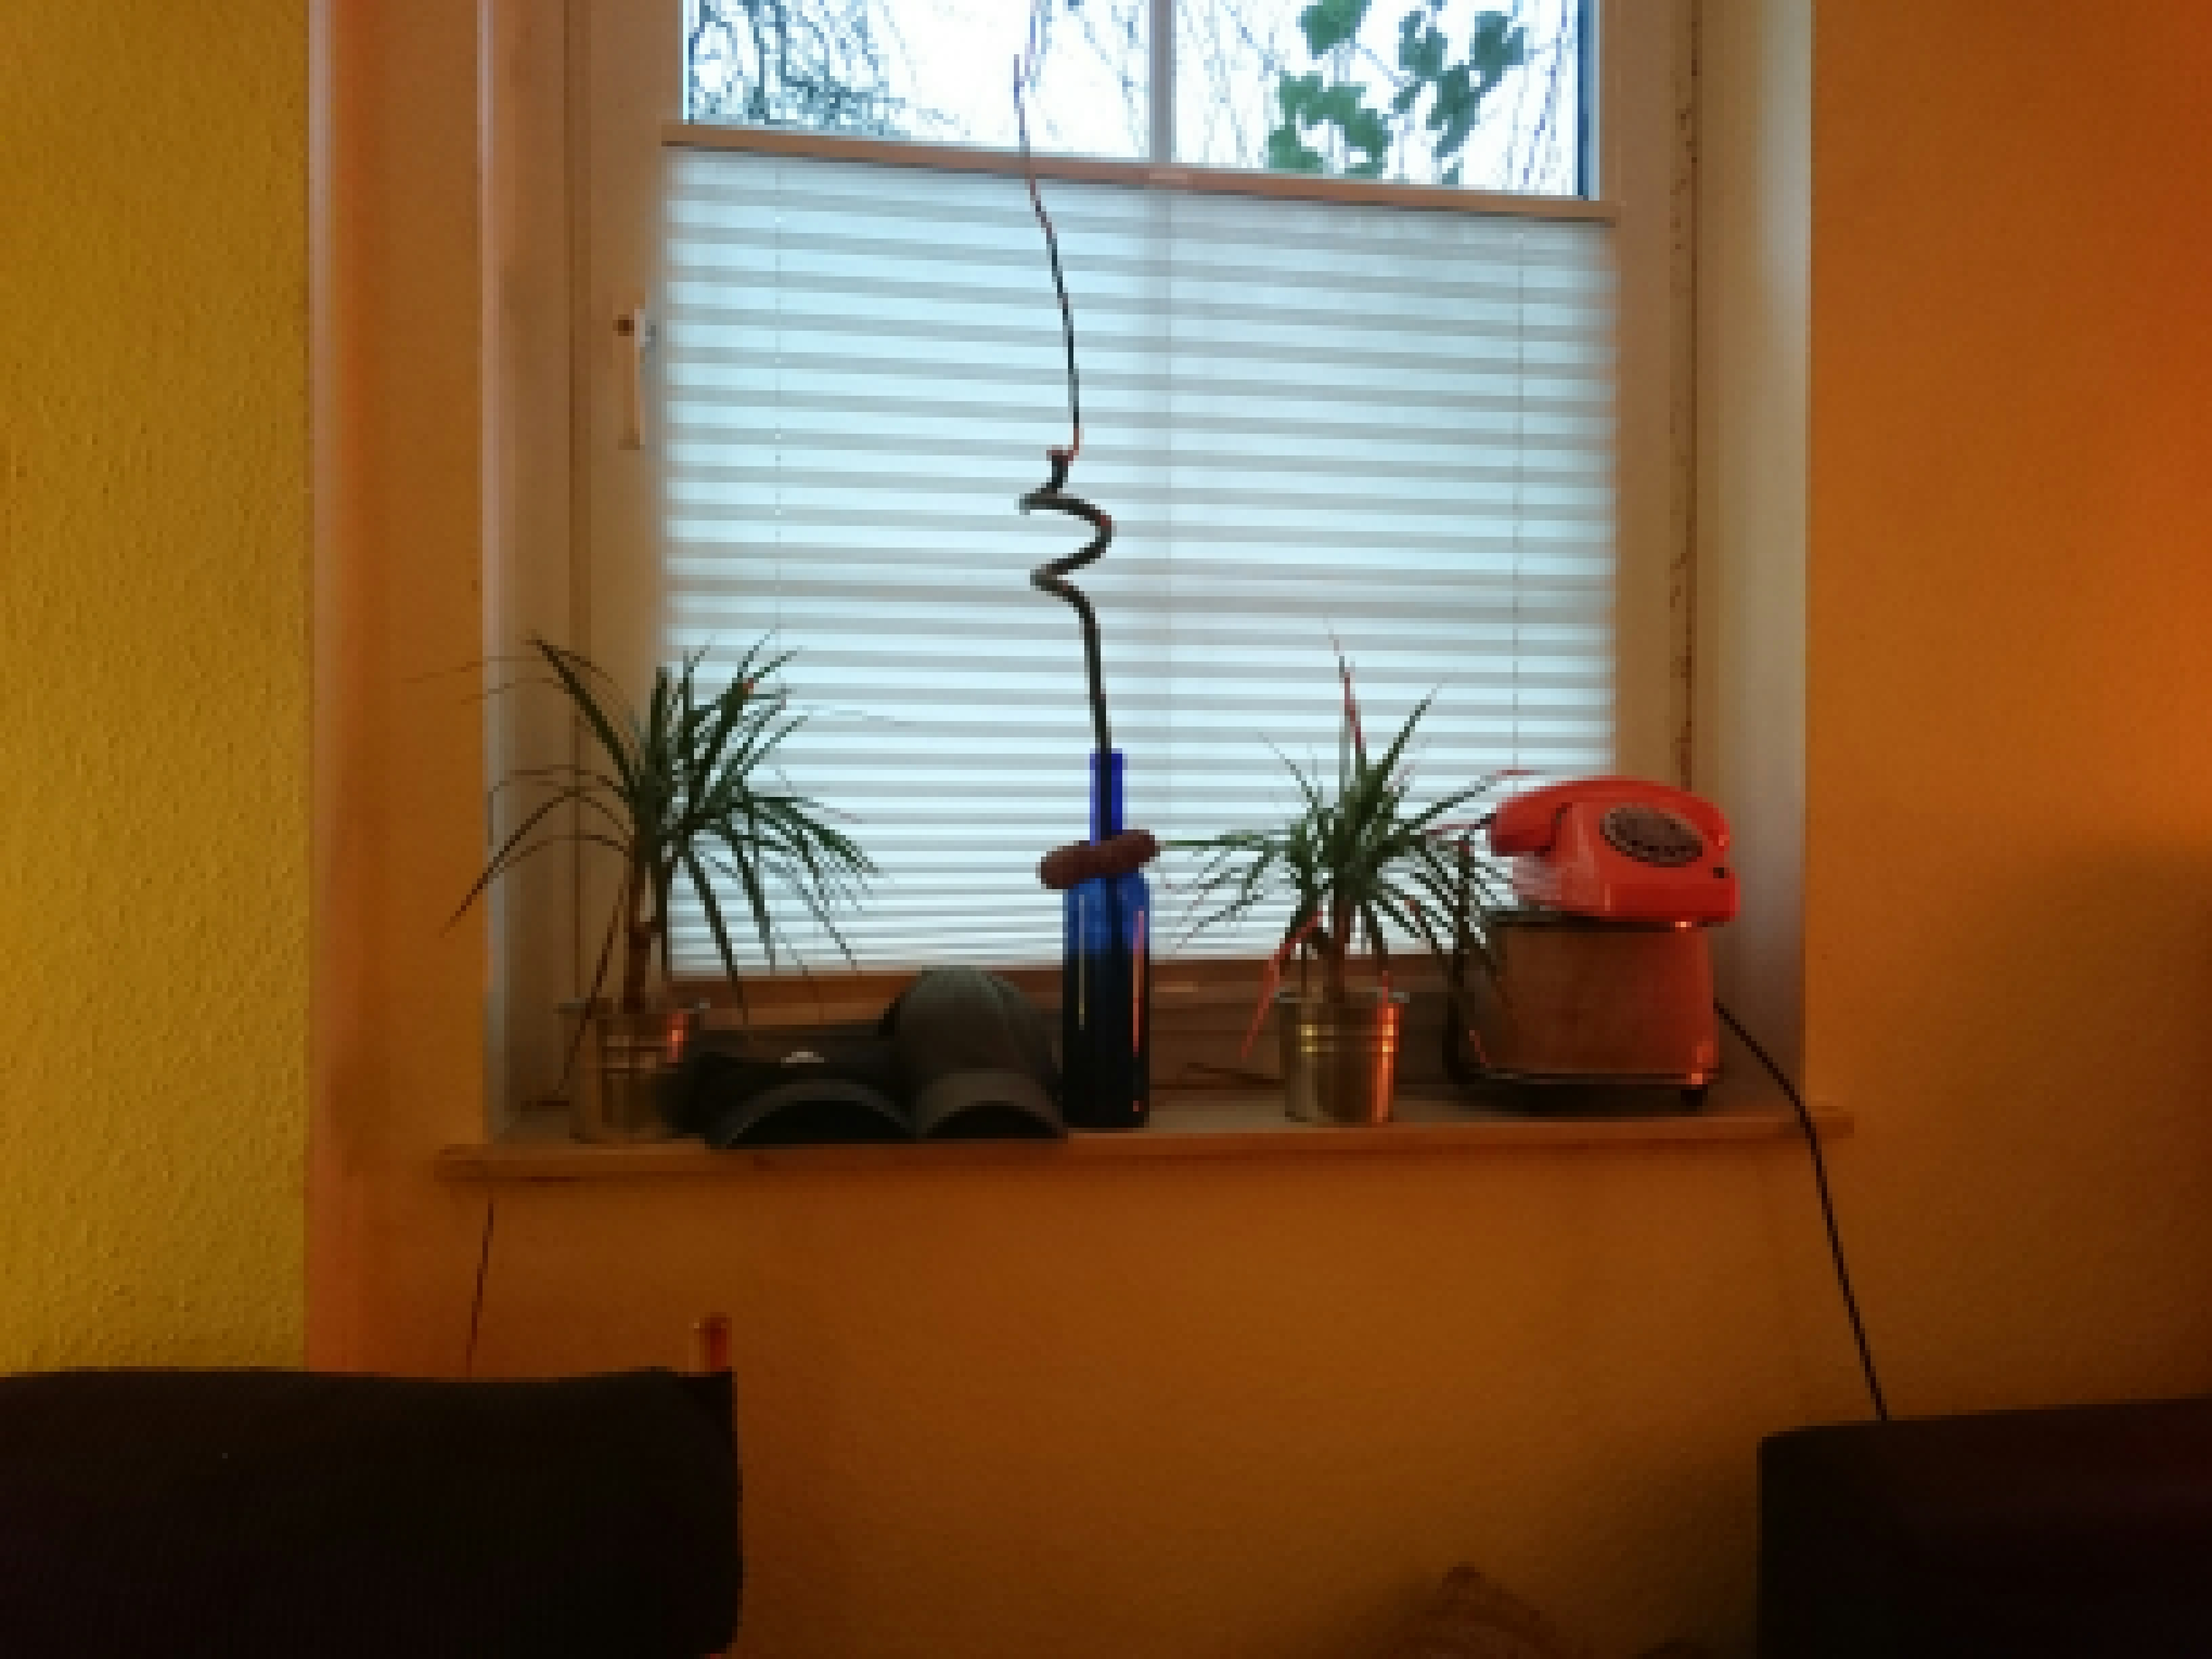
\includegraphics[width=1.4\textwidth]{img/Fotos/QuantiPig_Skalar_8x8.jpg}
	\caption[QuantiPig skalare Quantisierung 8x8 px]{QuantiPig skalare Quantisierung 8x8 px}
	\label{fig:pig_skalar 8x8}
\end{figure}

\begin{figure}[h]
	\centering
		
\includegraphics[width=1.4\textwidth]{img/Fotos/QuantiPig_Skalar_80x80.jpg}
	\caption[QuantiPig skalare Quantisierung 80x80 px]{QuantiPig skalare Quantisierung 80x80 px}
	\label{fig:pig_skalar 8x8}
\end{figure}


\end{landscape}


\clearpage

\subsection{Bildgrößen}
\begin{itemize}
	\item Original: 3,8 MB
	\item skalare Quantisierung:
		\begin{itemize}
			\item 2x2:	3,8 MB
			\item 4x4:	2,6 MB
			\item 8x8:	0,58 MB
			\item 80x80:0,12 MB 
		\end{itemize}
	\item Midtread: 4,9 MB
\end{itemize}













\section{Anhang}

